\documentclass{article}

\makeatletter
\def\and{%
  \end{tabular}%
  \begin{tabular}[t]{c}}
\makeatother


%\documentclass{llncs}
\newcommand{\inst}[1]{$^{#1}$}

\usepackage{minted}

\usepackage{amsmath}
\usepackage{amsthm}

%\theoremstyle{definition}
%\newtheorem{definition}{Definition}

\newenvironment{definition}{%
  \begin{quote}\textbf{Definition.}}{%
  \end{quote}}

\newcommand{\captionex}[2]{\caption[#1]{\textbf{#1.} #2}}


%\usepackage{squeeze_llncs}
\usepackage[left=1.6in,right=1.6in,top=1in,bottom=1in]{geometry}
\usepackage{changepage}
\usepackage{verbatim}
%\usepackage{times}

%\pagestyle{plain} % For page numbers
%\pagenumbering{arabic}

% \usepackage{ifthen}
% \usepackage{alltt}
% \usepackage{indentfirst}
\usepackage{latexsym}
\usepackage{amssymb}
\usepackage{graphicx}
% \usepackage{gdefs}
% \usepackage{logdef}
%\usepackage{setspace}
\usepackage{hhline}
\usepackage{refs}
% \usepackage{graph}
\usepackage{changebar}
\usepackage{multirow}
\usepackage{array}
% \usepackage{wrapfig}
% \usepackage[figuresright]{rotating}
\usepackage[figuresleft]{rotating}
\usepackage{color}
%\usepackage[noend]{algorithmic}
%\algsetup{indent=2em}
\usepackage[noline,noend]{algorithm2e}
%\usepackage{program}
\usepackage{paralist}
\usepackage{geometry}

\usepackage{hyperref}
\usepackage[all]{hypcap}

\usepackage{threeparttable}

\usepackage{misc}
% Using this for writing inference rules
\usepackage{mathpartir}

\usepackage{tikz}
\usetikzlibrary{snakes,arrows,shapes}

\usepackage[section,above]{placeins}
\usepackage[maxfloats=25]{morefloats}

\usepackage{adjustbox}
\usepackage{expdlist}
\usepackage{etoolbox}
\usepackage{settobox}
%\usepackage{ulem} % for strike out

\usepackage{afterpage}
\newcommand{\antistupidfloats}{\afterpage{\clearpage}}

\setcounter{topnumber}{5}
\def\topfraction{0.99}
\def\textfraction{0.05}
\def\floatpagefraction{0.9}
\setcounter{bottomnumber}{5}
\def\bottomfraction{0.99}
\setcounter{totalnumber}{10}
\def\dbltopfraction{0.99}
\def\dblfloatpagefraction{0.9}
\setcounter{dbltopnumber}{5}

\newlength{\defaultlabelsep}
\setlength{\defaultlabelsep}{\labelsep}

\usepackage{tweaklist}
% this sets the spacings in the itemize environment
\renewcommand{\itemhook}{\setlength{\topsep}{0pt}%
  \setlength{\itemsep}{0pt}%
  \setlength{\parsep}{0ex}%
}

% this sets the spacings in the enumerate environment
\renewcommand{\enumhook}{\setlength{\topsep}{0pt}%
  \setlength{\itemsep}{0pt}%
  \setlength{\parsep}{0ex}%
}


% this sets the spacings in the description environment
%\renewcommand{\descripthook}{\setlength{\topsep}{0pt}%
%  \setlength{\itemsep}{0pt}%
%  \setlength{\parsep}{0ex}%
%  \setlength{\labelsep}{\textwidth}%
%}


% \usepackage{relsize}

% \definecolor{highlight}{rgb}{.8,.8,.8}

\newcommand{\bottom}{\bot}

\newcommand{\toprule}{\hline}
\newcommand{\midrule}{\hline}
\newcommand{\bottomrule}{\hline}

%\setdescription{labelsep=\textwidth}


%%%%%%%%%%%%%%%%%%%

\let\oldthebibliography=\thebibliography
  \let\endoldthebibliography=\endthebibliography
  \renewenvironment{thebibliography}[1]{%
    \begin{oldthebibliography}{#1}%
      \setlength{\parskip}{0ex}%
      \setlength{\itemsep}{0ex}%
  }%
  {%
    \end{oldthebibliography}%
  }


%% Modified from http://anthony.liekens.net/index.php/LaTeX/MultipleFootnoteReferences
%% (I inserted the 'Footnote:' prefix)
%%
%% Use like:
%%    \footnoteremember{myfootnote}{This is my footnote}
%%    \footnoterecall{myfootnote}
\newcommand{\footnoteremember}[2]{
  \footnote{#2}
  \newcounter{Footnote:#1}
  \setcounter{Footnote:#1}{\value{footnote}}
}
\newcommand{\footnoterecall}[1]{
  \footnotemark[\value{Footnote:#1}]
}


\sloppy
\begin{document}
\pagestyle{plain}
\title{WALi: Nested-Word Automata
\thanks{\scriptsize Supported
by NSF under grants CCF-\{0540955, 0810053, 0904371\},
by ONR under grants N00014-\{09-1-0510, 10-M-0251\},
by ARL under grant W911NF-09-1-0413,
and by AFRL under grants FA9550-09-1-0279 and FA8650-10-C-7088.
Any opinions, findings, and conclusions or recommendations expressed
in this material are those of the author(s) and do not necessarily
reflect the views of the sponsoring agencies.
} 
}



\author{Evan Driscoll\inst{1} \and Aditya Thakur\inst{1} \and Amanda Burton\inst{1} \and Thomas Reps\inst{1,2}}
%\institute{
%  University of Wisconsin \and GrammaTech, Inc. \\
%  \email{\{burtona,adi,driscoll,reps\}@cs.wisc.edu}
%}
\date{}

%\begin{adjustwidth}{-.5in}{-.5in}
\maketitle
{\centering
\inst{1}University of Wisconsin --- Madison \\
Computer Sciences Department \\
\texttt{\{driscoll,adi,burtona,reps\}@cs.wisc.edu} \\
\vspace{\baselineskip}
\inst{2}GrammaTech, Inc.

}
%\end{adjustwidth}



\vspace{2\baselineskip}

%Tom's macros

%\addtolength{\topmargin}{-1.2in}       % move top margin up
%\setlength{\textwidth}{6.0in}
%\setlength{\oddsidemargin}{.25in}
%\setlength{\evensidemargin}{.25in}
%\addtolength{\textheight}{2.0in}

%\setcounter{topnumber}{5}
%\def\topfraction{0.99}
%\def\textfraction{0.05}
%\def\floatpagefraction{0.9}
%\setcounter{bottomnumber}{5}
%\def\bottomfraction{0.99}
%\setcounter{totalnumber}{10}
%\def\dbltopfraction{0.99}
%\def\dblfloatpagefraction{0.8}
%\setcounter{dbltopnumber}{5}

\setcounter{topnumber}{5}
\def\topfraction{0.99}
\def\textfraction{0.05}
\def\floatpagefraction{0.9}
\setcounter{bottomnumber}{5}
\def\bottomfraction{0.99}
\setcounter{totalnumber}{10}
\def\dbltopfraction{0.99}
\def\dblfloatpagefraction{0.9}
\setcounter{dbltopnumber}{5}

\newcommand{\pre}{\mbox{{\it pre\/}}}
\newcommand{\post}{\mbox{{\it post\/}}}
\newcommand{\Principals}{\mbox{{\rm Principals\/}}}
\newcommand{\Resources}{\mbox{{\rm Resources\/}}}
\newcommand{\Pair}[1]{\langle{#1}\rangle}
\renewcommand{\Vec}[1]{\overrightarrow{#1}}
\newcommand{\dV}{\delta V}
\newcommand{\dl}{\delta l}
\newcommand{\dW}{\delta W}

%%%%%%%%%%%%%%%%%%%%%%%%%%%%%%%%%%%%%%%%%%%%%%%%%%%%%%%%%%%%%%%%%%%%%%%%%

%%%% Greek and calligraphic letters %%%%%%%%%%%%%%%%%%%%%%%%%%%%%%%%%%%%%

\newcommand{\calA}{\mathcal A}
\newcommand{\calB}{\mathcal B}
\newcommand{\calC}{\mathcal C}
\newcommand{\calG}{\mathcal G}
\newcommand{\calI}{\mathcal I}
\newcommand{\calK}{\mathcal K}
\newcommand{\calM}{\mathcal M}
\newcommand{\calO}{\mathcal O}
\newcommand{\calP}{\mathcal P}
\newcommand{\calS}{\mathcal S}
\newcommand{\calW}{\mathcal W}
\newcommand{\calZ}{\mathcal Z}

% \newcommand{\Zsym}{\calZ}
% \newcommand{\Zsymb}{\calZ_\bot}
% \newcommand{\Zsymbt}{\calZ_\bot^\top}
\newcommand{\Zsym}{\mathbb{Z}}
\newcommand{\Zsymb}{\Zsym_\bot}
\newcommand{\Zsymbt}{\Zsym_\bot^\top}

\newcommand{\pproc}{\textit{p}}
\newcommand{\fproc}{\textit{f}}
\newcommand{\pmain}{\textit{main}}

\newcommand{\D}{\Delta}
\newcommand{\E}{\mathcal{E}}
\newcommand{\G}{\Gamma}
\newcommand{\Gr}{\calG}
\renewcommand{\P}{\calP}
\newcommand{\U}{\mathcal{U}}
\newcommand{\X}{\mathcal{X}}
\newcommand{\W}{\calW}

\renewcommand{\a}{\alpha}
\renewcommand{\d}{\delta}
\newcommand{\f}{\varphi}
\newcommand{\y}{\gamma}

\newcommand{\emptybox}{\square}
\newcommand{\fullbox}{\blacksquare}


\def\at#1{{\it AT}_{(#1)}}
\def\propagate#1{{\it propagate}(#1)}
\def\propagateprime#1{{\it propagate'}(#1)}
\def\update#1#2{{\it update}(#1,#2)}
\def\updateprime#1#2{{\it update'}(#1,#2)}
\def\updatewitness#1#2#3#4{{\it update}(#1,#2,#3,#4)}
\def\updatewitnessprime#1#2#3#4{{\it update'}(#1,#2,#3,#4)}
\def\heap{{\it heap}}

%%%% General use macros %%%%%%%%%%%%%%%%%%%%%%%%%%%%%%%%%%%%%%%%%%%%%%%%%

\def\Nseto{{\rm I\!N}_0}
\def\prestar{{{\it pre}^*}}
\def\poststar{{{\it post}^*}}
\def\autlang{L}
\def\ee{\varepsilon}

\def\rel{{\it rel}}
\def\trans{{\it trans}}
\def\eps{{\it eps}}

\def\gets{:=}

%%%% fillers %%%%%%%%%%%%%%%%%%%%%%%%%%%%%%%%%%%%%%%%%%%%%%%%%%%%%%%%%%%%

\def\Rightarrowfill{$\mathsurround0pt\smash\Relbar\mkern-7mu%
  \cleaders\hbox{$\mkern-2mu\smash\Relbar\mkern-2mu$}\hfill\mkern-7mu%
  \mathord\Rightarrow$}

\def\hookarrowfill{$\smash\lhook\mkern-5mu%
  \cleaders\hbox{$\mkern-2mu\smash\relbar\mkern-2mu$}\hfill\mkern-7mu%
  \mathord\rightarrow$}

%%%% all sorts of arrows %%%%%%%%%%%%%%%%%%%%%%%%%%%%%%%%%%%%%%%%%%%%%%%%

\def\genarrow#1#2#3#4{%
\mathrel{\smash{\setbox0=\hbox{$\scriptstyle{#1}$}%
\mathop{\setbox1=\hbox to \wd0{#4}%
\ht1=3pt\dp1=-2pt\box1}\limits^{#2}_{#3}}}}

%%%% single arrows %%%%%%%%%%%%%%%

% simple single arrow
\def\to{\rightarrow}

% single arrow with something on top
\def\tarrow#1{\genarrow{#1\quad}{#1}{}{\rightarrowfill}}

% single arrow with something below
\def\barrow#1{\genarrow{#1\quad}{}{#1}{\rightarrowfill}}

% single arrow with something on top and below
\def\tbarrow#1#2{\genarrow{#1\quad}{#1}{#2}{\rightarrowfill}}

% single arrow like before, but length is adapted to the lower inscription
\def\tbsymarrow#1#2{\genarrow{#2\quad}{#1}{#2}{\rightarrowfill}}

%%%% double arrows %%%%%%%%%%%%%%%

% simple double arrow
\newcommand{\da}{\Rightarrow}

% double arrow with something on top
\def\dtarrow#1{\genarrow{#1\quad}{#1}{}{\Rightarrowfill}}

% double arrow with something below
\def\dbarrow#1{\genarrow{#1\quad}{}{#1}{\Rightarrowfill}}

%%%% hook arrows %%%%%%%%%%%%%%%%%

% simple hook arrow
\newcommand{\hra}{\hookrightarrow}

% hook arrow with something on top
\def\hooktarrow#1{\genarrow{#1\quad}{#1}{}{\hookarrowfill}}

% hook arrow with something below in brackets
\def\hookbsymarrow#1{\genarrow{#1\quad\>}{}{[#1\,]}{\hookarrowfill}}

%%%%%%%%%%%%%%%%%%%%%%%%%%%%%%%%%%%%%%%%%%%%%%%%%%%%%%%%%%%%%%%%%%%%%%%%%

%%%% automata relations

\def\ausingle#1{\mathrel{\tarrow{#1}}}
\def\austar#1{\mathrel{\tarrow{#1}^*}}
\def\auplus#1{\mathrel{\tarrow{#1}^+}}
\def\austeps#1#2{\mathrel{\tbarrow{#1}{#2}}}
\def\ausingleindex#1#2{\mathrel{\tarrow{#1}_{#2}}}
\def\austarindex#1#2{\mathrel{\tarrow{#1}^*_{#2}}}

%%%% pushdown rules

\def\tup#1{\langle#1\rangle}
\def\pdrule#1#2{\tup{#1}\hra\tup{#2}}
\def\apdrule#1#2{\tup{#1}\hra\{#2\}}
\def\pdlabeledrule#1{\hooktarrow{#1}}
\def\pdruleindex#1#2#3{\tup{#1}\hra_{#2}\tup{#3}}

%%%% pushdown relations

\def\pdsingle{\mathrel{\da}}
\def\pdstar{\mathrel{\da^*}}
\def\pdplus{\mathrel{\da^+}}
\def\pdlabel#1{\mathrel{\dtarrow{#1}}}
\def\pdsteps#1{\mathrel{\dbarrow{#1}}}
\def\pdrep{\mathrel{\da^r}}

\def\pdsingleindex#1{\mathrel{\da_{#1}}}
\def\pdstarindex#1{\mathrel{\da^*_{#1}}}
\def\pdplusindex#1{\mathrel{\da^+_{#1}}}
\def\pdstepsindex#1#2{\mathrel{\dbarrow{#1}_{#2}}}

%%%%%%%%%%%%%%%%%%%%%%%%%%%%%%%%%%%%%%%%%%%%%%%%%%%%%%%%%%%%%%%%%%%%%%%%%

%%%% Algorithms

\newcounter{zeile}
\newbox\kasten
\setbox\kasten=\hbox{00}
\let\graph=\par
{\catcode`\[=\active\catcode`\>=\active
\gdef\addto#1#2{$#1:=#1\cup\{#2\}$}
\gdef\insertcombine#1#2#3{$#1 := #1~#2 \mapsto (#1(#2) \combine #3)~$}
\gdef\for#1{[for all] $#1$ [do]}
\gdef\addtrans{{\it add\_trans}}
\gdef\while#1{[while] $#1$ [do]}
\gdef\ifthen#1{[if] $#1$ [then]}
\gdef\endif{[f{}i]}
\gdef\od{[od]}
\gdef\algsetsize{}
\gdef\algo{\catcode`\~=\active
        \catcode`\[=\active\catcode`\>=\active\setcounter{zeile}{0}
        \def\par{\refstepcounter{zeile}\graph\noindent\kern\wd\kasten%
                \llap{{\small\thezeile}}\quad\algsetsize}
        \def[##1]{{\bf##1}}\def~##1~{\mathchar"405B##1\mathchar"505D}
        \def>{\quad}\obeylines}}

\newcounter{algcounter}
\def\newalgo#1{\refstepcounter{algcounter}\thealgcounter\label{#1}}
\def\defnewalgo#1{\refstepcounter{algcounter}\label{#1}}

%%%% Theorem-like environments

% \newtheorem{theorem}{Theorem}[section]
% \newtheorem{proposition}{Proposition}[section]
% \newtheorem{corollary}{Corollary}[section]
% \newtheorem{lemma}{Lemma}[section]
% \newtheorem{remark}{Remark}[section]
% \newtheorem{notation}{Notation}[section]
% \newtheorem{definition}{Definition}[section]
% \newtheorem{example}{Example}[section]
% \newtheorem{conjecture}{Conjecture}[section]
% \newenvironment{proof}{\noindent {\bf Proof:\,}}{\hfill$\;\;\Box$\medskip}

%%%% Symbols for labelling section

\def\lbot{0}
\def\ltop{1}
\def\srZero{\overline{0}}
\def\srOne{\overline{1}}
\def\combine{\oplus}
\def\extend{\otimes}
\def\bigcomb{\bigoplus}
\def\bigext{\bigotimes}
\def\mopval{\delta}
\def\witness{\omega}
\def\pval{v}
\def\tval{{\it val}}
\def\lle{\sqsubseteq}
\def\gle{\sqsupseteq}
\def\llt{\sqsubset}
\def\lmin{\min\nolimits_\lle}
\def\shortest{{\it minpath}}
\def\kderiv#1{\mathrel{\barrow{#1}}}

\newcommand{\Chi}{X}
\newcommand{\bigmeet}{\mathop\sqcap}
\def\bigmeet{\mathop{\rule[-0.2ex]{.07em}{2.17ex}
                \rule[1.8ex]{0.5em}{.17ex}
                \rule[-0.2ex]{.07em}{2.17ex}}}
% \def\bigmeet{\mathop{\mathchoice{\mbox{\rule[-1ex]{0.05em}{3.35ex}\rule[2.1ex]{0.8em}{0.1em}\rule[-1ex]{0.05em}{3.35ex}}}
%   {\mbox{\rule[-.5ex]{0.05em}{2.25ex}\rule[1.65ex]{.55em}{0.05em}\rule[-.5ex]{0.04em}{2.25ex}}}
%   {\mbox{\rule[-.5ex]{0.05em}{2.25ex}\rule[1.65ex]{.55em}{0.05em}\rule[-.5ex]{0.04em}{2.25ex}}}
%   {\mbox{\rule[-.5ex]{0.05em}{2.25ex}\rule[1.65ex]{.55em}{0.05em}\rule[-.5ex]{0.04em}{2.25ex}}}
% }}
%\newcommand{\bigtimes}{\mathop\times}
%\newcommand{\path}[2]{{\mathit path}(#1,#2)}

\newcommand{\wnode}{{\it wnode}}
\newcommand{\wstruc}{{\it wstruc}}
\newcommand{\nil}{{\it nil}}
\newcommand{\ta}{n}

\def\pdstepr#1{\mathrel{\dtarrow{\langle#1\rangle}}}
\def\pdsteprindex#1#2{\mathrel{\dtarrow{\langle#1\rangle}_{#2}}}
\def\pdlpath#1{\mathrel{\dbarrow{#1}^\extend}}
\def\pdlpartial#1{\mathrel{\dbarrow{#1}^\join}}

% %%%%%%%%%%%
% Nick's additions to macro(s)
\newcommand{\conf}[1]{\langle #1 \rangle}
\newcommand{\Rule}[2]{\conf{#1}\hookrightarrow\conf{#2}}
\def\SigmaE{\Sigma_{\epsilon}}
\def\dhat{\hat{\delta}}
\def\Apost{A_{\poststar}}
\def\deltai{\delta_{i}}
\def\deltac{\delta_{c}}
\def\deltar{\delta_{r}}
\def\deltain#1{\delta_{i|#1}}
\def\deltacn#1{\delta_{c|#1}}
\def\deltarn#1{\delta_{r|#1}}
\def\prefix#1#2{#1|_{#2}}
\def\cons{\kappa}
\def\nmain{n_{\text{main}}}
\def\NWofRun{\textit{NWofRun}}
\def\Runs{\textit{Runs}}
\def\GamA{\Gamma^{\alpha}}
\def\GamB{\Gamma^{\beta}}
\def\Lphi{L^{\varphi}}
\def\qerr{q_{\textit{err}}}
\def\sqalpha{\sqsubseteq_{\alpha}}
\def\Bool{\mathbb{B}}
\newcommand{\PA}[0]{\P_{A}}
\newcommand{\EffLen}[0]{\textit{EffLen}}
\def\run{\rho}
\def\build{\textit{build}}
\def\flatten{\textit{flatten}}
\def\vstep#1{v[#1]}
 % Contains various defs and macros for PDS notation
\newcommand{\merge}{\textit{merge}}
\newcommand{\projectOp}{\textit{project}}
\newcommand{\WPDS}{{\sc WPDS}}
\newcommand{\EWPDS}{\text{\sc EWPDS}}
\newcommand{\PDS}{\text{\sc PDS}}
\newcommand{\IMOP}{\text{\sc IMOP}}
\newcommand{\MFP}{\text{\sc MFP}}
\newcommand{\IMOVP}{\text{\sc IMOVP}}
\newcommand{\MOVP}{\text{\sc MOVP}}
\newcommand{\MOP}{\text{\sc MOP}}
\newcommand{\GPS}{\text{\sc GPS}}
\newcommand{\GPP}{\text{\sc GPP}}
\newcommand{\calR}{\text{\cal R}}
\newcommand{\AP}{\mathcal{AP}}
\newcommand{\ap}{\text{\it ap}}
\newcommand{\bind}{\text{\it bind}}
\newcommand{\mayalias}{\text{\it may-alias}}
\newcommand{\fooproc}{\text{\it foo}}
\newcommand{\barproc}{\text{\it bar}}
\newcommand{\state}[1]{\langle{#1}\rangle}
\newcommand{\matched}{\textit{matched}}
\newcommand{\valid}{\textit{valid}}

\newcommand{\transition}{\hookrightarrow}
\newcommand{\compose}{\circ}
\newcommand{\call}{\text{\it call}}
\newcommand{\retSite}{\text{\it return-site}}
\newcommand{\return}{\text{\it return}}
\newcommand{\enter}{\text{\it enter}}
\newcommand{\TotalCallSites}{\text{\it CallSites}}
\newcommand{\sem}[1]{[\![ #1 ]\!]}
\newcommand{\isem}[1]{[\![ #1 ]\!]^*}
\newcommand{\calN}{\mathcal N}
\newcommand{\calL}{\mathcal L}
\newcommand{\calE}{\mathcal E}
\newcommand{\gr}{\textit{ExGr}_v}
\newcommand{\Moped}{\text{\sc Moped}}
\newcommand{\exit}{\text{\it exit}}
\newcommand{\init}{\text{\it init}}
\newcommand{\proc}{\text{\it proc}}
\newcommand{\node}{\text{\it n}}
\newcommand{\head}{\texttt{head}}
\newcommand{\pop}{\text{\it pop}}
\newcommand{\grow}{\text{\it grow}}
\newcommand{\paths}{\text{\it paths}}
\newcommand{\push}{\text{\it push}}
\newcommand{\intraweight}{\text{\sc IntraQ}}
\newcommand{\moped}{\text{\sc Moped}}
\newcommand{\algs}{\text{\sc Alg0}}
\newcommand{\alga}{\text{\sc Alg1}}
\newcommand{\algb}{\text{\sc Alg2}}
\newcommand{\algc}{\text{\sc Alg3}}
\newcommand{\algd}{\text{\sc Alg4}}
\newcommand{\npoststar}{\text{\it poststar}}
\newcommand{\nprestar}{\text{\it prestar}}
\newcommand{\pdspath}[2]{{\mathit path}(#1,#2)}

\newcommand{\varx}{\texttt{x}}
\newcommand{\valx}{\overline{\texttt{x}}}
\newcommand{\pts}{\textsc{Pts}}
\newcommand{\vecspan}{\textsc{Span}}
\newcommand{\ip}{\text{\bf IP}}
\newcommand{\Val}{\text{Val}}
\newcommand{\Var}{\textit{Var}}
% Created by Tom, taken from FSTTCS submission

%\newcommand{\TODO}[1]{\textbf{[TODO #1]}}

\let\realincludegraphics\includegraphics
\renewcommand{\includegraphics}[2][Whatever]{}

%\newcommand{\nwaimage}[2][]{\realincludegraphics[#1]{#2}}
\newsavebox{\thenwaimagebox}
\newlength{\thenwaimagewidth}
\newlength{\thenwaimageheight}

\newcommand{\nwaimage}[2][0.66]{%
  \sbox{\thenwaimagebox}{\input{#2}}%
  \settoboxwidth{\thenwaimagewidth}{\thenwaimagebox}%
  \settoboxheight{\thenwaimageheight}{\thenwaimagebox}%
  %
  % If (width < textwidth) && (height < textheight)
  %    don't resize
  % else
  %    do resize
  %
  % except split this up for easier latexing
  %
  \ifdimless{\thenwaimagewidth}{#1\textwidth}{%
    \ifdimless{\thenwaimageheight}{#1\textheight}{%
      \usebox{\thenwaimagebox}%
    }{%
      \adjustbox{width=#1\textwidth,height=#1\textheight,keepaspectratio=true}{\usebox{\thenwaimagebox}}%
    }%
  }{%
    \adjustbox{width=#1\textwidth,height=#1\textheight,keepaspectratio=true}{\usebox{\thenwaimagebox}}%
  }%
}

\newenvironment{functionlist}%
               {\begin{list}{\TODO{MISSING}}{\setlength{\itemsep}{0pt}%
                                             \setlength{\parsep}{0ex}}}
               {\end{list}}
\newcommand{\functionitem}[1][\TODO{missing}]{\item[#1]\hspace*{\fill}\\}
\newcommand{\functionitemnonl}[1][\TODO{missing}]{\item[#1]}

\newcommand{\functionDef}[4]{\item[\texttt{#1 \textsl{#2}(#3) #4}]\mbox{}\\}
\newcommand{\functionDefEarly}[4]{\item[\texttt{#1 \textsl{#2}(#3) #4}]}
\newcommand{\functionDefFirst}[4]{\vspace{0.5\baselineskip}\item[\texttt{#1 \textsl{#2}(#3) #4}]\mbox{}\\}
\newcommand{\functionDefFirstEarly}[4]{\vspace{0.5\baselineskip}\item[\texttt{#1 \textsl{#2}(#3) #4}]}

\newcommand{\functionDefNoCloseParen}[3]{\item[\texttt{#1 \textsl{#2}(#3}]\mbox{}\\}
\newcommand{\functionDefEarlyNoCloseParen}[3]{\item[\texttt{#1 \textsl{#2}(#3}]}
\newcommand{\functionDefFirstNoCloseParen}[3]{\vspace{0.5\baselineskip}\item[\texttt{#1 \textsl{#2}(#3}]\mbox{}\\}
\newcommand{\functionDefFirstEarlyNoCloseParen}[3]{\vspace{0.5\baselineskip}\item[\texttt{#1 \textsl{#2}(#3}]}

\setlength{\belowcaptionskip}{0.66\baselineskip}

\newcommand{\wild}{\ensuremath{@}}
\renewcommand{\epsilon}{\varepsilon}

\section{Library Overview}
\label{Se:Nested Word Automata}

WALi-NWA is a C++ library for constructing, querying, and operating on
nested-word automata.  It is a portion of the WALi library, which provides
types and operations for weighted automata.
While the NWA portions of WALi
are mostly logically separate from the rest of WALi, it does use
facilities provided by WALi and inter-operates with WALi's weighted pushdown
system (WPDS) code.

We assume the reader is familiar with nested words and
nested-word automata; if not, \appref{nwa-definition} provides the definition
we use and
Alur et al.~\cite{DLT:AM2006,JACM:AM2009} describe them in detail. Our
implementation corresponds to the definition from the DLT 2006
paper~\cite{DLT:AM2006}; relative to followup work~\cite{JACM:AM2009}, this definition removes
the distinction between the machine's linear and hierarchical states, and on
a call transition always stacks the source state. In addition, we only require that the
final linear state be accepting for an NWA to accept a
word. (Following~\cite{JACM:AM2009}, this specific variant is a
``weakly-hierarchical, linearly-accepting'' NWA.)

The terminology used in the interface of the package is geared
toward program analysis, so we use terms such as ``call site'' and ``return
site'' to refer to states of the NWA even though they take on different
meanings in different contexts.

In contrast to the standard definitions, we allow internal $\epsilon$
transitions (but not calls or returns). We also allow ``wild''
transitions, which match any single symbol. (Wilds \emph{can} appear on calls
and returns.)

%The NWAs in this library have support for balanced and unbalanced-left nested
%words only, and does not provide support for any words with pending
%returns. (That is, we support balanced words and nested-word prefixes, but
%not nested-word suffixes or general nested words.)

The WALi library is available from
\url{http://www.cs.wisc.edu/wpis/wpds/download.php}. This document describes
the NWA portion of version 4.0. Building instructions can be found in
\texttt{README.txt} in the root directory of the distribution.

\clearpage
\tableofcontents
\clearpage

\subsection{Library overview}

The core of the NWA library is in the namespace \texttt{wali::nwa}. It
includes the classes \texttt{NestedWord}, \texttt{NWA}, and others.

There are a large number of non-member functions that operate on NWAs. These
are divided into three sub-namespaces:
\texttt{wali::nwa::query}, \texttt{wali::nwa::construct}, and
\texttt{wali::nwa::nwa\_pds}. There is also an experimental parser in
\texttt{wali::nwa}.

Finally, there are some operations and classes provided by WALi that the NWA
portion of the library uses. This mostly consists of the key-handling code,
but can also include the WPDS portions of the library.

Throughout this document, include paths are relative to the \texttt{Source}
directory from the WALi distribution.

\subsubsection{NWA core classes}

These types live in namespace \texttt{wali::nwa}:

\begin{functionlist}
  \functionitem[\texttt{NestedWord}] Implements a single nested word. Currently the only
    operation that can be performed using one is checking whether a
    \texttt{NestedWord} is a member of an \texttt{NWA}'s language. Defined in
    \texttt{wali/nwa/NestedWord.hpp}. See \sectref{class-nested-word}.
  \functionitem[\texttt{NWA}] Implements a nested-word automaton. Defined in
    \texttt{wali/nwa/NWA.hpp} with a forward declaration in \texttt{wali/nwa/NWAFwd.hpp}.
    See
    \sectref{NWA-class}. (\sectref{serialization} also discusses member
    functions related to serializing an NWA.)
  \functionitem[\texttt{NWARefPtr}] \texttt{NWARefPtr} is a typedef of \texttt{ref\_ptr$<$NWA$>$} (see
    below). This is defined in \texttt{wali/nwa/NWAFwd.hpp}.
  \functionitem[\texttt{State} and \texttt{Symbol}] These are both typedefs of
    \texttt{wali::Key} (see below). Both are defined in
    \texttt{wali/nwa/NWAFwd.hpp}. \emph{Note:} the use of keys for both
    states and symbols means that they can be confused from a types
    perspective, so use caution that this does not happen. 
  \functionitem[\texttt{StateSet} and \texttt{SymbolSet}] These are typedefs of
    \texttt{std::set}s of the corresponding type. (Client code should not
    rely on this
    fact; it could change to be an \texttt{unordered\_map} or other similar
    container.) Both are defined in \texttt{wali/nwa/NWAFwd.hpp}.
  \functionitem[\texttt{ClientInfo}] This class holds client-specific information that
    is associated with a state. Client code can subclass \texttt{ClientInfo} and use
    functions of the \texttt{NWA} class to attach instances to states. To use,
    include \texttt{wali/nwa/ClientInfo.hpp}. See \sectref{client-info}.
  \functionitem[\texttt{WeightGen}] This abstract class describes how to assign weights
    to transitions of the NWA, and is used both when converting an NWA to a
    PDS and when doing prestar/poststar queries on the NWA directly. To use,
    include \texttt{wali/nwa/WeightGen.hpp}. See \sectref{NWAtoPDS}.
\end{functionlist}


\subsubsection{NWA non-member functions}

The library provides a large number of non-member functions for operating on
NWAs. These are partitioned into the following namespaces:

\begin{functionlist}
  \functionitem[\texttt{wali::nwa::query}] This namespace provides functions for
    querying an automaton. The kinds of functions in this namespace are:
    \begin{itemize}
      \item Functions that query transitions of
        the NWA, returning information about one of the states or the symbol
        in transitions that meet some criteria. (For example, ``give me all
        states that appear as the target state of an internal transition with
        this source state.'') See \sectref{query-transitions}.
      \item Determining whether two NWAs have any states in
        common. See \sectref{query-automaton}.
      \item Determining whether an \texttt{NWA} is deterministic. See
        \sectref{query-automaton}.
      \item Determining whether a \texttt{NestedWord} is a member of the
        language of an NWA. See \sectref{query-language}.
      \item Determining whether the language of an NWA is empty. See
        \sectref{query-language}.
      \item Determining whether the languages of two NWAs are equal, or if
        one is a subset of the other. See \sectref{query-language}.
      \item prestar and poststar operations on an NWA. See
        \sectref{query-language}.
    \end{itemize}
    
  \functionitem[\texttt{wali::nwa::construct}] This namespace provides functions for
    constructing an NWA. Functions in this namespace are standard,
    automata-theoretic operations such as intersection, union, concatenation,
    Kleene star, and reversal. See \sectref{Building NWAs}.
  \functionitem[\texttt{wali::nwa::nwa\_pds}] This namespace provides functions for
    converting between NWAs and PDSs, and related functions. (Note that
    construction of an NWA from a PDS is in this namespace, not in
    \texttt{construct}.) See \sectref{Conversions}.
  \functionitem[\texttt{wali::nwa}] This namespace, in addition to the items already
    discussed, provides an experimental parser for a serialization format of
    NWAs. See \sectref{serialization}.
\end{functionlist}


\subsubsection{Generic WALi}

The NWA library uses these portions of the standard WALi library. Unless
otherwise specified, they are in namespace \texttt{wali}. See \cite{wali}.

\begin{functionlist}
  \functionitem[\texttt{ref\_ptr$<$T$>$}] This is a reference-counted, intrusive
    smart-pointer template. (``Intrusive'' means that the pointed-to type
    must be modified to include a \texttt{count} field used by the
    pointer. This is most conveniently done by subclassing
    \texttt{wali::Countable}.) Defined in \texttt{wali/ref\_ptr.hpp}.
  \functionitem[\texttt{Key}] A \texttt{Key} is a unique identifier naming states and symbols in an
    NWA or NestedWord. It is actually a typedef of an integer, though client
    code should not rely on this precise type. Declared in
    \texttt{wali/Key.hpp}.
  \functionitem[\texttt{getKey(...)}] This function produces a key from some input. If
    the input has not been seen before, it returns a new key; if it has, then
    it returns the same key as before. (One can think of this as translating
    whatever unique identifier is known by the client code to the
    \texttt{Key} needed by WALi.) Overloads of this function are provided for
    the following types:
    \begin{itemize}
      \item \texttt{std::string const \&}
      \item \texttt{char *}
      \item \texttt{int}
      \item \texttt{std::set<Key> const \&}
      \item \texttt{Key, Key} (this is a two-argument version of
        \texttt{getKey})
      \item \texttt{key\_src\_t}
    \end{itemize}

    The final overload, for \texttt{key\_src\_t}, is a \texttt{ref\_ptr} to a
    \texttt{KeySource} object. \texttt{KeySource} is an abstract class that
    client code can subclass to provide a translation to \texttt{Key}s for
    arbitrary types.

    All overloads are declared in \texttt{wali/Key.hpp}.
  \functionitem[\texttt{key2str}] \texttt{key2str} is an ``inverse'' of \texttt{getKey}, except that it
    always returns a string representation. If the key was created with
    \texttt{getKey(std::string const \&)} in the first place, this
    returns a copy of the original string.\footnote{For \texttt{int}s, it is the
    textual representation of the original number. For a \texttt{set<Key>},
    it is the set printed in standard set notation. For a pair of keys, it is
    the pair printed as an ordered pair. In general, it is the result of
    calling \texttt{key\_src\_t::print}. See the \texttt{print} function in
    each of the files \texttt{wali/*Source.cpp}.} Declared in
    \texttt{wali/Key.hpp}.
  \functionitem[\texttt{wali::wfa::WFA}] This is a weighted finite automaton. It is
    used in NWA poststar and prestar queries in much the same manner as in
    WPDS poststar and prestar queries. Defined in \texttt{wali/wfa/WFA.hpp}.
  \functionitem[\texttt{wali::wpds::WPDS}] This is a weighted pushdown system. NWAs use
    WPDSs behind the scenes when doing poststar and prestar queries, and the
    library provides conversion routines between the two automata
    types. Defined in \texttt{wali/wpds/WPDS.hpp}.
\end{functionlist}



\clearpage
\section{The \texttt{NestedWord} class}
\label{Se:class-nested-word}

The class \texttt{wali::nwa::NestedWord} is very simple. It provides support for
building nested words and iterating over their lengths; currently there
is no support for modifying them (other than appending).

The representation used by this class is closer to that of a word in a
visibly-pushdown language~\cite{JACM:AM2009}. It holds the linear contents of
a word, but does not store the nesting relation explicitly. Instead, each
position in the word is annotated with whether it is an internal, call, or
return position. The nesting relation is induced by the matchings between
calls and returns.

A position in the word is represented by the (nested) structure
\texttt{NestedWord::Position}. \texttt{Position} itself declares an
enumeration \texttt{Type} which is one of \texttt{CallType},
\texttt{InternalType}, or \texttt{ReturnType}.
A \texttt{Position} object has two (public) fields: \texttt{Symbol symbol}
and \texttt{Position::Type type}; these hold the symbol at that position and
the type of the position.


The \texttt{NestedWord} class has just six functions:
\begin{description}
  \item\texttt{appendInternal(Symbol s)}
  \item\texttt{appendCall(Symbol s)}
  \item\texttt{appendReturn(Symbol s)}
    These append the symbol \texttt{s} to the linear word, and annotate that
    position as an internal, call, or return position, respectively.
  \item\texttt{append(Position p)}
    Appends \texttt{p} to the word.
  \item\texttt{begin()}
  \item\texttt{end()}
    These return a \texttt{NestedWord::const\_iterator} to the start or end
    of the nested word. The type returned by dereferencing these iterators is
    a \texttt{Position} object. (There is no non-const version of these
    functions.)
\end{description}

The only operation the library currently supports on
\texttt{NestedWord}s, besides building them, is to check whether a
nested word is in an NWA's language. This is done by the function
\texttt{wali::nwa::query::languageContains}; see
\sectref{query-language}.


\clearpage
\section{The \texttt{NWA} class}
\label{Se:NWA-class}

\subsection{Construction, copying, and assignment}
\label{Se:Construction}

The NWA provides two constructors, the default constructor and the copy
constructor. The default constructor creates an empty NWA. Thereafter,
client code can add or remove states, add or remove symbols, add or remove
transitions, and set the status of certain states as initial or final.


The following functions are basic NWA operations:
\begin{functionlist}
  \functionitem[\texttt{NWA::NWA()}]
    Constructs an empty NWA.

  \functionitem[\texttt{NWA::NWA(NWA const \& other)}] Copies \texttt{other}; the
    automata will not share structure. Any client information that is present is cloned.

  \functionitem[\texttt{NWA::operator=(NWA const \& other)}] Assigns \texttt{other} to \texttt{this};
    the automata will not share structure.

  \functionitem[\texttt{NWA::clear()}] \nopagebreak
    Removes all states, symbols, and transitions from the NWA.

\end{functionlist}


\subsection{Simple manipulations}

An NWA object tracks the set of states, symbols, and transitions in the
automaton. It also tracks the set of initial and accepting states.
Counting each kind of transition separately, this gives 7 kinds of
``entities'' that client code may need to manipulate.

For each kind of entity, there are \texttt{NWA} member functions to add and
remove a single entity, check whether a particular entity is in the
automaton, count the number of entities of a particular type, remove all
entities of a particular type, and retrieve the set of entities in the
NWA. In addition, there are member functions for counting and clearing all
transitions, regardless of the type.

The names of these functions are very regular, but
\tableref{simple-functions} (\appref{Tables}) gives a list.

The only potential difficulties are in the interactions between the
functions. Naturally, removing a state or a symbol also removes all
transitions involving it; hence, clearing all states or clearing all symbols
also clears all transitions. (Calling \texttt{removeInitialState} or \texttt{removeFinalState}
does not cause ripple effects, however.)

Adding a transition implicitly adds the states and symbol involved in that
transition if they are not already present; hence it is not necessary to
explicitly add all states and symbols before adding transitions. (It is quite
reasonable to build an NWA by just adding initial states, final states, and
transitions.)


The system supports two meta-symbols: \texttt{wali::WALI\_EPSILON}
(\texttt{$\epsilon$}) and \texttt{wali::WALI\_WILD} (\texttt{\wild}).
\texttt{WALI\_EPSILON} is the standard $\epsilon$ from automata theory; it
denotes the situation in which a transition can be traversed without matching
and consuming an input symbol.  Epsilon symbols cannot label call or return
transitions. \texttt{WALI\_WILD} is the `any' symbol; it matches a single input
symbol of any kind.  Because the NWA alphabet is not fixed, the actual symbols
that \texttt{WALI\_WILD} stands for is fluid.  \textsl{Note:}
\texttt{WALI\_EPSILON} and \texttt{WALI\_WILD} are not explicit
elements of $\Sigma$; see \tableref{simple-functions}, footnote 5. \TODO{Fix
  footnote ref after modifying those in-table.}



\subsection{Client Information}
\label{Se:client-info}

Each state in the NWA can be associated with some client-specific
information. To utilize this functionality, client code must subclass
\texttt{ClientInfo} and override \texttt{ClientInfo * clone() const}.

Once done, client information can be attached or retrieved using the
following two functions (both members of \texttt{NWA}):
\begin{functionlist}
  \functionitem[\texttt{ref\_ptr<ClientInfo> NWA::getClientInfo( Key st ) const}]
    Allows the user to access the client-specific information associated with
    the given state, \texttt{st}.
  \functionitem[\texttt{void NWA::setClientInfo( Key st, ref\_ptr<ClientInfo> ci )}]
    Allows the user to specify the client-specific information, \texttt{ci},
    associated with the given state, \texttt{st}. \\
\end{functionlist}
Client information is tracked through the use of \texttt{ref\_ptr}s, so the
programmer must consider the standard aliasing and lifetime considerations
imposed by using smart pointers.

\vspace{\baselineskip}
In addition, you may wish to subclass \texttt{NWA} itself. There are several
virtual helper functions that are called during intersection and
determinization to compute the client info for the resulting automaton; these
can be overriden to customize the behavior. (This design is an instance
of the ``template method'' design pattern.)

The list of these helper methods is:
\begin{itemize}
  \item \texttt{intersectClientInfoInternal}
  \item \texttt{intersectClientInfoCall}
  \item \texttt{intersectClientInfoReturn}
  \item \texttt{mergeClientInfo}
  \item \texttt{mergeClientInfoInternal}
  \item \texttt{mergeClientInfoCall}
  \item \texttt{mergeClientInfoReturn}
\end{itemize}
(The first three are used by intersection and the remaining four by
determinization.) In addition, \texttt{stateIntersect} and
\texttt{transitionIntersect} can further customize the behavior of
intersection, including computation of client
information. \sectrefs{Intersection}{Determinize} have more information on
intersection and determinization, and discuss these functions further.


\begin{comment}

\subsection{The following are more functions that don't fit into the above categories}

\begin{functionlist}
  \functionitem[\texttt{void NWA::duplicateState( Key orig, Key dup )}] \nopagebreak

    Duplicates all the transitions containing the state \texttt{orig} and
    adds the transitions to the NWA with \texttt{orig} replaced by
    \texttt{dup}.  Self-loops are duplicated by adding a transition for all
    possible combinations of some occurrence of \texttt{orig} replaced by
    \texttt{dup}, i.e., if $(\texttt{orig},a,\texttt{orig})$ is an internal
    (or call) transition, then the transitions
    $(\texttt{dup},a,\texttt{dup})$, $(\texttt{dup},a,\texttt{orig})$, and
    $(\texttt{orig},a,\texttt{dup})$ are added and if
    $(\texttt{orig},\texttt{orig},a,\texttt{orig})$ is a return transition,
    then the transitions $(\texttt{dup},\texttt{dup},a,\texttt{dup})$,
    $(\texttt{dup},\texttt{dup},a,\texttt{orig})$,
    $(\texttt{orig},\texttt{dup},a,\texttt{dup})$,
    $(\texttt{orig},\texttt{dup},a,\texttt{orig})$,
    $(\texttt{dup},\texttt{orig},a,\texttt{dup})$,
    $(\texttt{dup},\texttt{orig},a,\texttt{orig})$, and
    $(\texttt{orig},\texttt{orig},a,\texttt{dup})$ are added.

  \functionitem[\texttt{void NWA::duplicateStateOutgoing( Key orig, Key dup )}] \nopagebreak

    Duplicates all the transitions originating from \texttt{orig} and adds
    the transitions to the NWA with \texttt{orig} replaced by \texttt{dup}.
    Self-loops are duplicated by adding a transition for all possible
    combinations of some occurrence of \texttt{orig} replaced by \texttt{dup}
    while maintaining that the transitions are outgoing from \texttt{dup},
    i.e., if $(\texttt{orig},a,\texttt{orig})$ is an internal (or call)
    transition, then the transitions $(\texttt{dup},a,\texttt{dup})$ and
    $(\texttt{dup},a,\texttt{orig})$ are added and if
    $(\texttt{orig},\texttt{orig},a,\texttt{orig})$ is a return transition,
    then the transitions $(\texttt{dup},\texttt{dup},a,\texttt{dup})$,
    $(\texttt{dup},\texttt{dup},a,\texttt{orig})$,
    $(\texttt{dup},\texttt{orig},a,\texttt{dup})$, and
    $(\texttt{dup},\texttt{orig},a,\texttt{orig})$ are added.

  \functionitem[\texttt{void NWA::realizeImplicitTrans(State stuck)}] \nopagebreak

    Makes the transition relation ``at least total.''
    For any source state and symbol pair that does not have at least one
    transition, adds a transition to \texttt{stuck}. It does the same for
    call transitions and return transitions (with an additional ``for each
    call predecessor'' for returns).

    Note that if the machine was nondeterministic, it will still be
    nondeterministic after this call.

\end{functionlist}

\end{comment}

\clearpage
\section{The \texttt{wali::nwa::query} namespace}
\label{Se:namespace-query}

The \texttt{wali::nwa::query} namespace provides functions related to
querying the structure of an automaton itself as well as various questions
based on its language.

In this section, we first discuss how to retrieve information from an
automaton's transitions (\sectref{query-transitions}) then move on to other
queries about an automaton proper.
Following that, we discuss queries about the
\textsl{language} of an automaton (\sectref{query-language}).


\subsection{Querying information from an automaton's transitions}
\label{Se:query-transitions}
The \texttt{wali::nwa::query} namespace provides a large number of functions
for retrieving information about an \texttt{NWA}'s transitions. The questions
answered by these functions are of the form ``what are all symbols that
appear on a return transition where the call predecessor state is \texttt{s1}
and the return site state is \texttt{s1}?''

Functions return information either about all transitions or about
transitions of a particular type (internal, call, or return). The names of
these functions have regular patterns based on the information that is
known and desired, but the rules for producing the names are perhaps not as
simple as they could be. Because of this,
Tabs.~\ref{Ta:query-all-transitions}--\ref{Ta:query-return-transitions}
provide a quick-lookup of the functions.

The tables do not have \textsl{all} the information one needs to know in
order to call them, and the entries use some shorthand; but they provide enough
information the specifics can be
looked up in the header or Doxygen documentation. The caption of each table
gives the header that contains the functions listed. In the interest of
space, the types of the function arguments are omitted, but they are likely to
be what you expect. (The number of arguments is also always sufficient to
uniquely identify the function since all types are just \texttt{wali::Key}s
anyway.) Almost all functions return a \texttt{StateSet}, \texttt{SymbolSet},
or a \texttt{std::set} of pairs of a state and a symbol. (Those that return a
set of pairs are marked specially.)

%To use the table to answer the question above, we first look at the table for
%return transitions (\tableref{query-return-transitions}). We know the call
%predecessor and return site, so we find the corresponding row in the table
%(fourth from the bottom). We want to know all the symbols, so we look at the
%symbol column. We see there are two choices: \texttt{getReturnSym\_CallRet}
%and \texttt{getExits}. By looking at \texttt{returns.hpp} or Doxygen
%documentation, we can see that the former returns a \texttt{SymbolSet}, which
%is what we want. The latter returns
%a \texttt{std::set$<$std::pair$<$State,Symbol$>>$}, which contains the
%information we desire, but is likely to be less convenient to
%use. (The \texttt{State} component of each pair is the exit site, which is
%where the function name \texttt{getExits} comes from.)



%\newcolumntype{x}[1]{p{#1}}
\newcommand{\RP}{\tnote{1}} %"returns pair"

\setlength{\extrarowheight}{4pt}

\newgeometry{bottom=0.75in,top=0.75in}

\begin{sidewaystable}\sffamily
\begin{threeparttable}
\begin{tabular}{p{1in}p{1in}|@{\hspace{0.1in}}p{2.2in}p{2.2in}p{2in}}
\toprule\toprule
\multicolumn{2}{c|@{\hspace{0.1in}}}{\textsl{What you know}} & \multicolumn{3}{c}{\textsl{What you want}}                                                                 \tabularnewline
 this...        & ... and this      &    sources                    &   symbols                          &    targets                     \tabularnewline
\midrule
\midrule %-------------------------------------------------------------------------------------------------------------------------------
  source        &  (nothing)        &      ---                      &  (none)                            &  getSuccessors(nwa, src)       \tabularnewline
                &  symbol           &      ---                      &        ---                         &  getSuccessors(nwa, src, sym)  \tabularnewline
                &  target           &      ---                      &  getSymbol(nwa, src, tgt, \&sym)   &   ---                          \tabularnewline
\midrule %-------------------------------------------------------------------------------------------------------------------------------
  symbol        &  (nothing)        &                               &        ---                         &   (none)                       \tabularnewline
                &  target           & getPredecessors(nwa, sym, tgt)&       ---                         &   ---                          \tabularnewline
\midrule %-------------------------------------------------------------------------------------------------------------------------------
  target        &  (nothing)        & getPredecessors(nwa, tgt)     &  (none)                            &   ---                          \tabularnewline
\bottomrule\bottomrule
\end{tabular}
\caption{\textbf{Query functions for all transitions.} These functions are
  in the namespace \texttt{wali::nwa::query}; include the
  file \texttt{wali/nwa/query/transitions.hpp}. For return transitions, the
  ``source'' is the first component of the transition; nothing involving call
  predecessors (the second component) appears in this sidewaystable. A table
  entry of ``---'' means that square does not make sense. }
\end{threeparttable}
\label{Ta:query-all-transitions}
\end{sidewaystable}

\begin{sidewaystable}\sffamily
\begin{threeparttable}
\begin{tabular}{p{1in}p{1in}|@{\hspace{0.1in}}p{2.2in}p{2.2in}p{2in}}
\toprule\toprule
\multicolumn{2}{c|@{\hspace{0.1in}}}{\textsl{What you know}} & \multicolumn{3}{c}{\textsl{What you want}}                                                                 \tabularnewline
 this...        & ... and this      &    sources                    &   symbols                          &    targets                     \tabularnewline
\midrule
\midrule %-------------------------------------------------------------------------------------------------------------------------------
 (nothing)      &  (nothing)        & getSources(nwa)               &  getInternalSym(nwa)               &  getTargets(nwa)               \tabularnewline
\midrule %-------------------------------------------------------------------------------------------------------------------------------
  source        &  (nothing)        &      ---                      &  getInternalSym\_Source(nwa, src) \newline
                                                                       or getTargets(nwa, src)\RP        &  getTargets(nwa, src)\RP       \tabularnewline
                &  symbol           &      ---                      &        ---                         &  getTargets(nwa, src, sym)     \tabularnewline
                &  target           &      ---                      &  getInternalSym(nwa, src, tgt)     &   ---                          \tabularnewline
\midrule %-------------------------------------------------------------------------------------------------------------------------------
  symbol        &  (nothing)        & getSources\_Sym(nwa, sym)     &        ---                         &  getTargets\_Sym(nwa, sym)     \tabularnewline
                &  target           & getSources(nwa, sym, tgt)     &        ---                         &   ---                          \tabularnewline
\midrule %-------------------------------------------------------------------------------------------------------------------------------
  target        &  (nothing)        & getSources(nwa, tgt)\RP       &  getInternalSym\_Target(nwa, tgt) \newline
                                                                       or getSources(nwa, tgt)\RP        &   ---                          \tabularnewline
\bottomrule\bottomrule
\end{tabular}
\begin{tablenotes}
  \item[1] Returns a set of pairs (either source/symbol or symbol/target).
\end{tablenotes}
\caption{\textbf{Query functions for internal transitions.}
  These functions are in the namespace \texttt{wali::nwa::query};
  include the file \texttt{wali/nwa/query/internals.hpp}.
  A table entry of ``---'' means that square does not make
  sense.}
\label{Ta:query-internal-transitions}
\end{threeparttable}
\end{sidewaystable}

\begin{sidewaystable}\sffamily
\begin{threeparttable}
\begin{tabular}{p{1in}p{1in}|@{\hspace{0.1in}}p{2.2in}p{2.2in}p{2in}}
\toprule\toprule
\multicolumn{2}{c|@{\hspace{0.1in}}}{\textsl{What you know}} & \multicolumn{3}{c}{\textsl{What you want}}                                                                 \tabularnewline
 this...        & ... and this      &    call sites                   &   symbols                          &    entries                     \tabularnewline
\midrule
\midrule %-------------------------------------------------------------------------------------------------------------------------------
 (nothing)      &  (nothing)        & getCallSites(nwa)               &  getCallSym(nwa)                   &  getEntries(nwa)               \tabularnewline
\midrule %-------------------------------------------------------------------------------------------------------------------------------
 call site      &  (nothing)        &      ---                        &  getCallSym\_Call(nwa, call)\newline
                                                                         or getEntries(nwa, call)\RP       &  getEntries(nwa, call)\RP      \tabularnewline
                &  symbol           &      ---                        &        ---                         &  getEntries(nwa, call, sym)    \tabularnewline
                &  target           &      ---                        &  getCallSym(nwa, call, ent)        &   ---                          \tabularnewline
\midrule %-------------------------------------------------------------------------------------------------------------------------------
  symbol        &  (nothing)        & getCallSites\_Sym(nwa, sym)     &        ---                         &  getEntries\_Sym(nwa, sym)     \tabularnewline
                &  target           & getCallSites(nwa, sym, ent)     &        ---                         &   ---                          \tabularnewline
\midrule %-------------------------------------------------------------------------------------------------------------------------------
  entry         &  (nothing)        & getCallSites(nwa, ent)\RP       &  getCallSym\_Entry(nwa, ent) \newline
                                                                         or getCallSites(nwa, ent)\RP      &   ---                          \tabularnewline
\bottomrule\bottomrule
\end{tabular}
\begin{tablenotes}
  \item[1] Returns a set of pairs (either call site/symbol or symbol/entry).
\end{tablenotes}
\caption{\textbf{Query functions for call transitions.} These functions are in the
  namespace \texttt{wali::nwa::query}; include the
  file \texttt{wali/nwa/query/calls.hpp}. The ``call site'' is the source of the transition (and uses the argument 
  name \texttt{call}), and the ``entry'' of the transition is the target (and
  uses the argument name \texttt{ent}). }
\label{Ta:query-call-transitions}
\end{threeparttable}
\end{sidewaystable}

\begin{sidewaystable}\footnotesize\sffamily
\begin{threeparttable}
\begin{tabular}{p{0.6in}p{0.65in}p{0.6in}|@{\hspace{0.1in}}p{1.75in}p{1.9in}p{1.9in}p{2in}}
\toprule\toprule
\multicolumn{3}{c|@{\hspace{0.1in}}}{\textsl{What you know}}  & \multicolumn{4}{c}{\textsl{What you want}}                                                                                                                                                \tabularnewline
 this...  & and this ...  & and this & exit sites & call predecessors &
 symbols & return sites \tabularnewline
\midrule
\midrule %--------------------------------------------------------------------------------------------------------------------------------------------------------------------------------------------------------------------
 (nothing)      &  (nothing)        &  (nothing)    & getExits(nwa)                 &  getCalls(nwa)                        &  getReturnSym(nwa)                           &  getReturns(nwa)                            \tabularnewline
\midrule %--------------------------------------------------------------------------------------------------------------------------------------------------------------------------------------------------------------------
 exit site      &  (nothing)        &  (nothing)    &      ---                      &  getCalls\_Exit(nwa, exit)\RP         &  getReturnSym\_Exit(nwa, exit) \newline
                                                                                                                               or getReturns\_Exit(nwa, exit)\RP\newline
                                                                                                                               or getCalls\_Exit(nwa, exit)\RP             &  getReturns\_Exit(nwa, exit)\RP             \tabularnewline
                \cline{2-7} %-------------------------------------------------------------------------------------------------------------------------------------------------------------------------------------------------
                &  call pred        &  (nothing)    &      ---                      &    ---                                &  getReturnSym\_ExitCall(nwa, exit, \newline
                                                                                                                               \phantom{getReturnSym\_ExitCall(}call) \newline
                                                                                                                               or getReturns(nwa, exit, call)\RP           &  getReturns(nwa, exit, call)\RP             \tabularnewline
                &                   &  symbol       &      ---                      &    ---                                &        ---                                   &  getReturns(nwa, exit, call, sym)           \tabularnewline
                &                   &  return       &      ---                      &    ---                                &  getReturnSym(nwa, exit, call, \newline
                                                                                                                               \phantom{getReturnSym(}ret)                 &    ---                                      \tabularnewline
                \cline{2-7} %-------------------------------------------------------------------------------------------------------------------------------------------------------------------------------------------------
                &  symbol           &  (nothing)    &      ---                      &  getCalls\_Exit(nwa, exit, sym)       &        ---                                   &  getReturns\_Exit(nwa, exit, sym)           \tabularnewline
                &                   &  return       &      ---                      &  getCalls(nwa, exit, sym, ret)        &        ---                                   &  getEntries(nwa, call, sym, ret)            \tabularnewline
                \cline{2-7} %-------------------------------------------------------------------------------------------------------------------------------------------------------------------------------------------------
                &  return site      &  (nothing)    &      ---                      &  getCalls(nwa, exit, ret)\RP          &  getReturnSym\_ExitRet(nwa, exit, \newline
                                                                                                                               \phantom{getReturnSym\_ExitRet(}ret) \newline
                                                                                                                               or getCalls(nwa, exit, ret)\RP              &   ---                                       \tabularnewline
\midrule %-------------------------------------------------------------------------------------------------------------------------------------------------------------------------------------------------------------------
 call pred      &  (nothing)        &  (nothing)    & getExits\_Call(nwa, call)\RP  &   ---                                 &  getReturnSym\_Call(nwa, call) \newline
                                                                                                                               or getReturns\_Call(nwa, call)\RP\newline
                                                                                                                               or getExits\_Call(nwa, call)\RP            &  getReturnSites(nwa, call) or \newline
                                                                                                                                                                             getCallSuccessors(nwa, call) or \newline
                                                                                                                                                                             getReturns\_Call(nwa, call)\RP              \tabularnewline
                \cline{2-7} %-------------------------------------------------------------------------------------------------------------------------------------------------------------------------------------------------
                &  symbol           &  (nothing)    & getExits\_Call(nwa, call, sym)&   ---                                 &        ---                                   &  getCallSuccessors(nwa, call, sym) \newline
                                                                                                                                                                              or getReturns\_Call(nwa, call, sym)        \tabularnewline
                &                   &  return       & getExits(nwa, call, sym, ret) &   ---                                 &        ---                                   &    ---                                      \tabularnewline
                \cline{2-7} %-------------------------------------------------------------------------------------------------------------------------------------------------------------------------------------------------
                &  return site      &  (nothing)    & getExits(nwa, call, ret)\RP   &   ---                                 &  getReturnSym\_CallRet(nwa, call, \newline
                                                                                                                               \phantom{getReturnSym\_CallRet(}ret) \newline
                                                                                                                               or getExits(nwa, call, ret)\RP              &   ---                                       \tabularnewline
\midrule %--------------------------------------------------------------------------------------------------------------------------------------------------------------------------------------------------------------------
 symbol         &  (nothing)        &  (nothing)    & getExits\_Sym(nwa, c)         &  getCalls\_Sym(nwa, c)                &   ---                                        &  getReturns\_Sym(nwa, sym)                  \tabularnewline
                \cline{2-7} %-------------------------------------------------------------------------------------------------------------------------------------------------------------------------------------------------
                &  return site      &  (nothing)    & getExits\_Ret(nwa, call, ret) &  getCallPredecessors(nwa, sym, ret) \newline
                                                                                       or getCalls\_Ret(nwa, sym, c)        &   ---                                        &   ---                                       \tabularnewline
\midrule %--------------------------------------------------------------------------------------------------------------------------------------------------------------------------------------------------------------------
 return site    &  (nothing)         & (nothing)    & getExits\_Ret(nwa, ret)       &  getCallPredecessors(nwa, ret) \newline
                                                                                       or getCalls\_Ret(nwa, ret)\RP        &  getReturnSym\_Ret(nwa, ret) or \newline
                                                                                                                               getCalls\_Ret(nwa, ret)\RP                  &   ---                                       \tabularnewline
\bottomrule\bottomrule
\end{tabular}
\begin{tablenotes}
  \item[1] Returns a set of pairs (a symbol with one of the states, in the order of the raw transition).
\end{tablenotes}
\caption{\textbf{Query functions for call transitions.} These functions are in the
  namespace \texttt{wali::nwa::query}; include the
  file \texttt{wali/nwa/query/returns.hpp}.   The ``exit site'' is the source of the transition
  (the first component) and uses the argument name \texttt{exit} in this table;
  the ``call predecessor'' is the second component and uses the argument
  name \texttt{call}; the symbol is the third component uses the argument
  name \texttt{sym}; the ``return site'' is the fourth component and uses the
  argument name \texttt{ret}. }
\label{Ta:query-return-transitions}
\end{threeparttable}
\end{sidewaystable}
\restoregeometry


\subsection{Querying other physical aspects of an automaton}
\label{Se:query-automaton}

The NWA library has two additional functions for querying attributes
of NWAs themselves. One computes whether an NWA is deterministic, and
the other computes whether two automata have any states in common.

These functions are declared in the header
\texttt{wali/nwa/query/automata.hpp} (and, of course, defined in the
namespace \texttt{wali::nwa::query}).

\begin{description}
  \item\texttt{bool isDeterministic(NWA const \& nwa)}
    Computes whether the given NWA is deterministic and returns the
    result. \textit{Warning:} The result is not cached in the NWA, and
    as presently-implemented, this function is very
    inefficient. Improvements to this will come in a later version of
    the library.
  \item\texttt{bool statesOverlap(NWA const \& a, NWA const \& b)}
    Comptuers whether the two NWAs share any states and returns the
    result.
\end{description}

\TODO{Should I even put isDeterministic() in there? I think it's
  pretty bad. I could fix it, but I'd like to get this out.}

\subsection{Querying properties of an automaton's language}
\label{Se:query-language}

The NWA library has several functions for querying standard
formal-language theoretic properties, and in addition supports
the poststar and prestar queries used in program analysis.

The functions that perform standard language-theoretic queries are
located in namespace \texttt{wali::nwa::query} and are declared in
\texttt{wali/nwa/query/language.hpp}. They are:
\begin{description}
  \item\texttt{bool languageContains(NWA const \& nwa, Nested Word
    const \& word)} Computes whether \texttt{word} is a member of
    \texttt{nwa}'s language, and returns the result. (It simulates the
    NWA in a nondeterministic fashion, so there is no determinization
    done.)
  \item\texttt{bool languageIsEmpty(NWA const \& nwa)} Computes
    whether the NWA's language is empty, and returns the result.
  \item\texttt{bool languageSubsetEq(NWA const \& left, NWA const \& right)}
    Computes whether $L(\texttt{left}) \subseteq L(\texttt{right})$
    and returns the result.
  \item\texttt{bool languageEquals(NWA const \& left, NWA const \& right)} 
    Equivalent to \texttt{languageSubsetEq(left, right) \&\&
    languageSubsetEq(right, left)}
\end{description}

Finally, there are functions for performing a poststar and prestar
query on an NWA. These work by converting the NWA to a WPDS (see
\sectref{Conversions} and, in particular, \sectref{NWAtoPDS}) using
\texttt{NWAtoPDScalls} then running the query on the PDS.

There are two variants of each. One returns the WFA that results from
the query, and the other stores the WFA in an output parameter. The
\texttt{WFA} type is \texttt{wali::wfa::WFA}.

The functions that perform poststar and prestar are in the namespace
\texttt{wali::nwa::query} and are declared in the header
\texttt{wali/nwa/query/weighted.hpp}. They are:
\begin{description}
  \item\texttt{WFA prestar( NWA const \& nwa, WFA \& input, WeightGen \& wg )}
  \item\texttt{void prestar( NWA const \& nwa, WFA \& input, WFA \& output, WeightGen \& wg )}
    Computes the prestar of the configurations specified by
    \texttt{input}, using the weights generated by \texttt{wg}. Either
    returns the result or stores it in the parameter \texttt{output}.
  \item\texttt{WFA poststar( NWA const \& nwa, WFA \& input, WeightGen \& wg )}
  \item\texttt{void poststar( NWA const \& nwa, WFA \& input, WFA \& output, WeightGen \& wg )}
    Computes the poststar of the configurations specified by
    \texttt{input}, using the weights generated by \texttt{wg}. Either
    returns the result or stores it in the parameter \texttt{output}.
\end{description}

\TODO{Check to see if I can make input and wg const.}

\clearpage
\section{NWA serialization}

\begin{comment}

It is possible to serialize an NWA in two different supported
formats.

The first is a description language of our own creation, described in
most of the rest of this section. We also provide a parser, with minor
caveats, for this format. The grammar the parser uses is defined
formally in \sectref{nwa-grammar}.

The second is output in Graphviz Dot format. The output is
natural. The color of an edge denotes the type of a transition: black
edges are internal transitions, green edges are call transitions, and
red edges are return transitions. Return transitions are labeled with
both the symbol for that transition and the call predecessor. (The
result of each Dot graph includes a key as a reminder for what the
colors mean.) Because it is possible to wind up with extremely long
key names (especially in a determinized NWA) that can essentially
destroy any ability of Dot to render useful output, by default any
state names longer than 20 characters are replaced by the numerical
value; this behavior can be changed however.

There is a member function which produces both types of output:
\begin{description}
  \item\texttt{std::ostream\& NWA::print(std::ostream \& stream) const}
    Writes the custom output described in this section
    to \texttt{stream}, returning \texttt{stream}.
    (This method is actually inherited from
    the \texttt{wali::Printable} abstract class.)

  \item\texttt{std::ostream\& NWA::print\_dot(std::ostream \& stream,
    std::string const \& name, bool abbreviate = true)} Outputs a Dot
    description of the NWA to the given stream. The name of the graph
    (\textsl{digraph "blah" \{...}) is given
    by \texttt{name}. Finally, if \texttt{abbreviate} is set
    to \texttt{false}, the abbreviation step above for state names is
    not done. Use this freedom at your peril.
\end{description}

\subsection{Parser}
\label{Se:parser}

The NWA library contains a semi-experimental parser for descriptions of
NWAs. The format is described below, and matches the result of calling
\texttt{NWA::print(std::ostream \&)}, provided that the result of
calling \texttt{key2str} on the state and symbol keys produces strings
that match the description of \textsl{actual-names} in this grammar.

There are two functions which parse NWA descriptions:
\begin{itemize}
  \item\texttt{NWARefPtr read\_nwa(std::istream \&, std::string * name = NULL)}
  \item\texttt{std::map$<$std::string, NWARefPtr$>$ read\_nwa\_proc\_set(std::istream \&)}
\end{itemize}
A stream may contain descriptions of one or more automata; the first
function reads one, and the second function reads all.  (The return
type of the second function has a typedef name of
\texttt{ProcedureMap}.)

The former function reads the first description of an NWA from the
input string and returns it. Descriptions specify an optional name of
an NWA; if one is specified and \texttt{name} is non-null, then the
name is stored in the string pointed to by \texttt{name}.

The second function reads the entire input stream. It returns a map
from the name of each automaton specification to the parsed NWA. (This
form was originally created to read NWAs for an entire program, witch
each procedure in a separate NWA. The name of each NWA was the name of
the procedure in the original program.)

\subsection{Examples}

The following are examples of the NWA serialization format, showing
both the general form and some of the flexibilities in what precise
format is accepted.

Exa:nwa-simple
 Q: { a }
 Q: b
 Delta\_i: (a, b (c), c)
 Delta\_i: (a, b, d)
 Delta\_r: (a, b, c, d)
 Delta\_c: {}


Exa:nwa-from-mattf
 Q: {
   (key\#6,3) (=16),
   (key\#6,4) (=17),
   (key\#7,3) (=18),
   (key\#4,3) (=19),
   (key\#3,3) (=20),
   (key\#5,3) (=21),
   (key\#9,3) (=22),
   (key\#5,4) (=23),
   (key\#9,4) (=24),
   (key\#10,3) (=25),
   (key\#10,4) (=26)
 }
 Q0: {
   (key\#6,3) (=16),
   (key\#6,4) (=17)
 }
 Qf: {
   (key\#5,4) (=23),
   (key\#9,4) (=24),
   (key\#10,4) (=26)
 }
 Sigma: {
   <start;0;expression>,
   <start;1;body;0>,
   <start;2;expression;1>,
   <{\#fun634}>,
   <start;2;expression>
 }
 Delta\_c: {
   ((key\#4,3) (=19) ,<{\#fun634}>, (key\#3,3) (=20) )
 }
 Delta\_i:  {
   ((key\#6,3) (=16) ,<start;0;expression>, (key\#7,3) (=18) ),
   ((key\#6,4) (=17) ,<start;0;expression>, (key\#7,3) (=18) ),
   ((key\#7,3) (=18) ,<start;2;expression;1>, (key\#4,3) (=19) ),
   ((key\#9,3) (=22) ,<start;2;expression>, (key\#10,3) (=25) ),
   ((key\#9,3) (=22) ,<start;2;expression>, (key\#10,4) (=26) ),
   ((key\#9,4) (=24) ,<start;2;expression>, (key\#10,3) (=25) ),
   ((key\#9,4) (=24) ,<start;2;expression>, (key\#10,4) (=26) )
 }
 Delta\_r: {
   ((key\#3,3) (=20) , (key\#4,3) (=19) ,<start;1;body;0>, (key\#5,3) (=21) ),
   ((key\#3,3) (=20) , (key\#4,3) (=19) ,<start;1;body;0>, (key\#9,3) (=22) ),
   ((key\#3,3) (=20) , (key\#4,3) (=19) ,<start;1;body;0>, (key\#5,4) (=23) ),
   ((key\#3,3) (=20) , (key\#4,3) (=19) ,<start;1;body;0>, (key\#9,4) (=24) )
 }

\subsection{NWA description format}
\label{Se:nwa-grammar}

This section describes the grammar of the file format.

\textsl{Note:} Some characteristics in the following have the
following as part of their description: ``you should not depend on
this.'' In such cases, we reserve the right to change this behavior in
future versions and to not feel bad about it.

\textsl{Note:} This is experimental code; in particular, the
error-handling in it is basically non-existent. We detect when the
input doesn't match the grammar, but we signal such input failures
with assertion violations. In a future version of the library, we will
report errors more gracefully, almost certainly through exceptions.

\textsl{Note:} The NWA parser has unit tests embedded in the code. (It
does not use any unit test framework.) These tests can be run by
calling \texttt{wali::nwa::parser\_test\_all}. The file
\texttt{NwaParserMain.cpp} is a short program that does this.


The grammar for an NWA is as follows. In order to accept a couple
slightly different output formats we have used in the past, there are
some choices in whether braces are present and other aspects.


A single input stream can contain either a single NWA (just a series
of blocks) or multiple NWAs. If you would like to describe multiple
NWAs, each individual starts with the literal \textsl{nwa}.

\end{comment}

\newenvironment{grammar}{\begin{equation*}\begin{array}{lrl}}{\end{array}\end{equation*}}
\newcommand{\nonterm}[1]{\ensuremath{\langle}\textit{#1}\ensuremath{\rangle}}
\newcommand{\term}[1]{\textrm`\texttt{#1}\textrm'}
\newcommand{\cfgsp}{\ \ }

\begin{grammar}
  \nonterm{nwa-description} & ::= & \left(\term{nwa}\cfgsp\nonterm{name}?\cfgsp\term{:}?\right)?\cfgsp\term{\{}?\cfgsp\nonterm{block}{+}\cfgsp\term{\}}?
\end{grammar}

\textsl{Braces are required if 'nwa' is present and the name is absent}
 in order to
 distinguish the first block header (\textsl{Q:}, \textsl{Q0:},
 or \textsl{Qf:}) from the name of the NWA.

An NWA is a sequence of blocks; each block specifies one or more
states, symbols, or transitions.

\begin{grammar}
  \nonterm{block} &  ::= & \nonterm{state-block} \\
                  &    | & \nonterm{sigma-block} \\
                  &    | & \nonterm{delta-block}
\end{grammar}

Blocks of the same type can be repeated; e.g. it is perfectly fine to
specify all transitions in one block (as in \exref{nwa-from-mattf},
one block per transition (as in \exref{nwa-simple}), or
anywhere in between. The ``block header'' specifies what kind of block
it is, and the body is a comma-separated list of whatever entity the
block header specifies (e.g. states). The body may be surrounded by
curly braces, but they are not required unless the body is empty.

If a block specifies states, it can specify just that a state is
present, an initial state, or an accepting state; these are denoted by
the block headers \textsl{Q:}, \textsl{Q0:}, and \textsl{Qf:}
respectively.
 
\begin{grammar}
  \nonterm{state-block} &  ::= & \term{Q:} \cfgsp \term\{? \cfgsp \nonterm{name-list}\cfgsp\term\}? \\
                        &   |  & \term{Q0:}\cfgsp \term\{? \cfgsp \nonterm{name-list}\cfgsp\term\}? \\
                        &   |  & \term{Qf:}\cfgsp \term\{? \cfgsp \nonterm{name-list}\cfgsp\term\}?
\end{grammar}

(It is not necessary to explicitly list all states; if a state is
listed in a transition, it is implicitly added to the machine if
needed. Thus it is quite possible to have a machine description with
no \textsl{Q:} blocks.)

A name-list is simply a comma-separate list of names of states.

\begin{grammar}
  \nonterm{name-list} & ::= & (\nonterm{name}\cfgsp (\term{,}\cfgsp  \nonterm{name})*)?
\end{grammar}

Recall that If the list is empty, it must be followed by a \textsl{\}}
(or EOF) to distinguish the next block header from the name of a
state.

The grammar for \textsl{name} will be specified below.


Symbol blocks are just like name blocks, except they specify symbol
names. The block header is simply 'sigma'.

\begin{grammar}
  \nonterm{sigma-block} & ::= & \term{sigma:}\cfgsp  \term{\{}?\cfgsp  \nonterm{name-list}\cfgsp  \term{\}}?
\end{grammar}

A transition block can be for internal, call, or return transitions,
denoted by the block headers \textsl{delta\_i}, \textsl{delta\_c}, and
\textsl{delta\_r}, respectively.
 
\begin{grammar}
  \nonterm{delta-block} & ::= & \term{delta\_i:}\cfgsp  \term{\{}?\cfgsp  \nonterm{triple-list}\cfgsp  \term{\}}? \\
                        &   | & \term{delta\_c:}\cfgsp  \term{\{}?\cfgsp  \nonterm{triple-list}\cfgsp  \term{\}}? \\
                        &   | & \term{delta\_r:}\cfgsp  \term{\{}?\cfgsp  \nonterm{quad-list}  \cfgsp  \term{\}}?
\end{grammar}

The bodies in each case are simply a comma-separated list of triples
or quads:

\begin{grammar}
  \nonterm{triple-list} & ::= & (\nonterm{triple}\cfgsp  (\term{,}\cfgsp  \nonterm{triple})*)? \\
  \nonterm{quad-list}   & ::= & (\nonterm{quad}\cfgsp  (\term{,}\cfgsp  \nonterm{quad})*)?
\end{grammar}

and each triple (resp., quad) is a 3-tuple (4-tuple) of names:

\begin{grammar}
  \nonterm{triple} & ::= &  \term{(}\cfgsp  \nonterm{name}\cfgsp \term{,}\cfgsp  \nonterm{name}\cfgsp  \term{,}\cfgsp  \nonterm{name}\cfgsp  \term{)} \\
  \nonterm{quad} & ::= &  \term{(}\cfgsp  \nonterm{name}\cfgsp \term{,}\cfgsp  \nonterm{name}\cfgsp  \term{,}\cfgsp  \nonterm{name}\cfgsp  \term{,}\cfgsp  \nonterm{name}\cfgsp  \term{)}
\end{grammar}


All that remains is to define the grammar for `name'. Because the
format grew organically and we wished to keep compatibility with
existing log files (which could previously not be automatically parsed
but which we could look at), the `name' terminal is a bit convoluted.

The name consists of the \textsl{actual} name of the state or symbol
in question, followed by an optional parenthesis-delimited token which
is ignored. (In some of our output, the name is the result of
\texttt{key2str} and the optional token is the actual numeric value of
the key.)

\begin{grammar}
  \nonterm{name} & ::= &  \nonterm{actual-name}\cfgsp  \nonterm{dummy-token}?
\end{grammar}

The actual-name portion generally behaves like a standard-programming
language identifier, but with one important difference: it can contain
balanced parentheses, and \textsl{any} characters are allowed within a
set of parentheses. (We actually allow a larger set of characters than
is typical, but you should not depend on this. Surround your names
with parentheses if you use ``special'' characters.)

We can now define the effective grammar. A `unit' is a letter or
parenthesis group.

\begin{grammar}
  \nonterm{actual-name} & ::= &  \nonterm{unit}+ \\
&& \\
  \nonterm{unit} & ::= &  \nonterm{normal-char} \\
                 &   | &  \nonterm{paren-group} \\
&& \\
  \nonterm{normal-char}& ::= &  \textrm{character other than whitespace, \term{,}, or a paren}
\end{grammar}

(\texttt{std::isspace} is used to determine whether a character is
  whitespace.)

\begin{grammar}
  \nonterm{left-paren}  & ::= &  \term{(}\cfgsp |\cfgsp \term{\{}\cfgsp |\cfgsp \term{[}\cfgsp |\cfgsp \term{$<$} \\
  \nonterm{right-paren} & ::= &  \term{)}\cfgsp |\cfgsp \term{\}}\cfgsp |\cfgsp \term{]}\cfgsp |\cfgsp \term{$>$} \\
  \nonterm{non-paren} & ::= &  \textrm{a character other than any of the above} \\
&& \\
  \nonterm{paren-group}& ::= &  \nonterm{left-paren}\cfgsp  (\nonterm{non-paren}\ |\ \nonterm{paren-group})*\cfgsp  \nonterm{right-paren}
\end{grammar}

(Finally, we do not currently demand that the \textsl{types} of parens
  match up: e.g. \texttt{(1, 2, 3]} is a valid name. You should not
    depend on this feature.)

\clearpage
\section{Building NWAs from other NWAs (namespace \texttt{wali::nwa::construct})}
\label{Se:Building NWAs}

The library provides functions for performing automata-theoretic operations upon
NWAs. The supported operations are union, intersection, concatenation,
reversal, Kleene star, complement, and determinization.

The library supports two interfaces to each of these operations. In one, the
operation allocates an NWA with \texttt{new}, performs the construction, and
returns a \texttt{NWARefPtr} to the result.  In the other, the operation takes
a reference to an NWA, clears it, and constructs the result in-place. The
first form is usually more convenient to use, and creates a mini language for
set expressions; the second form makes it possible to store the result of an
operation in a subclass of \texttt{NWA}.

Each of these functions is in the namespace \texttt{wali::nwa::construct}:

\begin{functionlist}

  \functionDefEarly{NWARefPtr}{unionNWA}{NWA const \& a, NWA const \& b}{}
  \functionDef{void}{unionNWA}{NWA \& out, NWA const \& a, NWA const \& b}{}
    Computes the union of the NWAs \texttt{a} and \texttt{b},
    either returning the result or storing it in \texttt{out}.
    See Section
    \ref{Se:Union}. (This function is called \texttt{unionNWA} instead of
    \texttt{union} because the latter is a C++ keyword.) The two NWAs must not
    have any states in common, and the output will be nondeterministic even
    if both input NWAs are deterministic. The running time\footnote{We count
      state lookups, additions, etc. as constant time even though they are
      actually logarithmic, and occasionally linear.} is
    $O(|Q^a|+|Q^b|+|\delta^a|+|\delta^b|)$.

  \functionDefFirstEarly{NWARefPtr}{intersect}{NWA const \& a, NWA const \& b}{}
  \functionDef{void}{intersect}{NWA \& out, NWA const \& a, NWA const \& b}{}
    Computes the intersection of the NWAs \texttt{a} and \texttt{b},
    either returning the result or storing it in \texttt{out}.
    See Section \ref{Se:Intersection}. If both input NWAs are deterministic,
    the output will be deterministic. The worst-case running time is
    $O(|Q^a| |Q^b| d_a d_b)$, where $d_a$ is the maximum out-degree
    of a state in \texttt{a} and $d_b$ is the maximum out-degree of a state
    in \texttt{b}.

  \functionDefFirstEarly{NWARefPtr}{concat}{NWA const \& left, NWA const \& right}{}
  \functionDef{void}{concat}{NWA \& out, NWA const \& left, NWA const \& right}{}
    Computes the concatenation of the NWAs \texttt{left} and
    \texttt{right}, either returning the result or storing it in
    \texttt{out}.
    See Section \ref{Se:Concatenation}. The output automaton will be
    nondeterministic. The running time is
    $O(|Q^a|+|Q^b|+|\delta^a|+|\delta^b|+|Q^a||\delta_r^b|)$.

  \functionDefFirstEarly{NWARefPtr}{star}{NWA const \& orig}{}
  \functionDef{void}{star}{NWA \& out, NWA const \& orig}{}
    Computes the Kleene star of the NWA \texttt{orig}, either
    returning the result or storing it in \texttt{out}. See Section
    \ref{Se:Star}. The output automaton will be nondeterministic. The
    running time is $O(|Q|+|\delta|+|Q_0||Q_f||\delta_c|)$.

  \functionDefFirstEarly{NWARefPtr}{reverse}{NWA const \& orig}{}
  \functionDef{void}{reverse}{NWA \& out, NWA const \& orig}{}
    Computes the NWA that accepts the reverse of each nested word
    accepted by the NWA \texttt{orig}, either returning the result or
    storing it in \texttt{out}. See Section \ref{Se:Reverse}. The running
    time is $O(|Q|+|\delta|)$.

  \functionDefFirstEarly{NWARefPtr}{determinize}{NWA const \& orig}{}
  \functionDef{NWARefPtr}{determinize}{NWA \& out, NWA const \& orig}{}
    Computes a determinization of \texttt{orig}, either returning the
    result or storing it in \texttt{out}.
    See Section \ref{Se:Determinize}. The worst-case running time for this
    algorithm is at least $O({|Q|^3} \cdot2^{|Q|^2})$.

  \functionDefFirstEarly{NWARefPtr}{complement}{NWA const \& orig}{}
  \functionDef{void}{complement}{NWA \& out, NWA const \& orig}{}
    Computes the complement of the determinization of \texttt{orig},
    either returning the result or storing it in \texttt{out}.
    See Section
    \ref{Se:Complement}. %For complementing the set of final states to work
    %correctly, two things must hold: \texttt{orig} must be deterministic and
    %the transition functions must be total. (That is, for a given state $q$
    %and symbol $\sigma$, there must be exactly one internal transition $(q,
    %5\sigma, q') \in\delta_i$, exactly one call transition $(q, \sigma,
    %q')\in\delta_c$, and exactly one return transition $(q, p, \sigma,
    %q')\in\delta_r$ for each state $p$.)
    \texttt{complement()} determinizes \texttt{orig}, so its worst-case
    running time is also at least $O({|Q|^3} \cdot2^{|Q|^2})$.

    %\vspace{0.5\baselineskip}
    %If \texttt{determinize} is \texttt{true}, it will
    %automatically determinize the input NWA before complementation, which
    %also guarantees the input machine will be total. If you
    %know that \texttt{orig} is already deterministic and total, you can set
    %\texttt{determinize} to
    %\texttt{false} to avoid this step. (Complementing a nondeterministic or
    %non-total NWA can easily lead to an incorrect result.) If
    %\texttt{determinize} is \texttt{true}, the worst-case running time is the
    %same as for the \texttt{determinize} function (roughly
    %$O(2^{|Q|^2})$). If \texttt{determinize} is \texttt{false}, the running
    %time is $O(|Q|+|\delta|)$.

\end{functionlist}

As mentioned above, these functions create a small language of set
expressions. For instance, to compute an automaton \texttt{M} whose language
is $\texttt{A} \cup (\texttt{B} \cap \texttt{C})*$ (where \texttt{A},
\texttt{B}, and \texttt{C} are \texttt{NWARefPtr}s), one can write
\begin{center}
  \texttt{NWARefPtr M = unionNWA(*A, *star(*intersect(*B, *C)))}
\end{center}


\begin{figure}[tb]
  \centering
  \begin{minipage}{0.49\textwidth}
    \centering
    \nwaimage[.49]{Figures/figure-1}
    \caption{An example NWA.}
    \label{Fi:Example1}
  \end{minipage}
  \begin{minipage}{0.49\textwidth}
    \centering
    \nwaimage[0.49]{Figures/union-other}
    \caption{A second example NWA.}
    \label{Fi:Union1}
  \end{minipage}
\end{figure}

\begin{figure}[tbp]
  \centering
    \nwaimage[.55]{Figures/union-result}
  \caption{The NWA resulting from the union of the NWA in Figure
    \ref{Fi:Example1} and the NWA in Figure \ref{Fi:Union1}. Note that there
    are two initial states.}
  \label{Fi:Union2}
\end{figure}



\subsection{Union}
\label{Se:Union}
The union of two NWAs is constructed by taking the union of each of the
components of the NWAs. (In
particular, it does \textsl{not} do a cross-product construction, and will
\textsl{always} produce a nondeterministic automaton as a result as long as
both machines have at least one initial state.)

Formally, given $N$ and $M$ such that
\begin{itemize}
 \item $N = (Q_N, \Sigma_N, Q_{0,N}, \delta_N, F_N)$
 \item $M = (Q_M, \Sigma_M, Q_{0,M}, \delta_M, F_M)$
\end{itemize}
then the union is computed as follows:
\begin{itemize}
 \item $N \cup M = (Q_N \cup Q_M, \Sigma_N \cup \Sigma_M, Q_{0,N} \cup
   Q_{0,M}, \delta_N \cup \delta_M, F_N \cup F_M)$
\end{itemize}

As an example, \figref{Union2} illustrates the union of \figref{Example1} and
\figref{Union1}.


The state sets of the NWAs must not overlap,
i.e., $Q_1 \cap Q_2 = \emptyset$. \textsl{Client code should not rely on
  this condition being checked} or any particular behavior occurring if it
does not hold.

Client information is copied directly from the original NWAs using
\texttt{ClientInfo::clone()}.


\subsection{Intersection}
\label{Se:Intersection}

The intersection of two NWAs is computed in the standard cross-product
fashion, using a worklist algorithm to only compute those states that
are reachable.

The algorithm traverses the original NWAs starting at
the initial states and incrementally adds transitions for each pair of
``intersectable'' transitions that are encountered. By default, transitions
are intersectable when the transitions are the same kind (internal, call,
or return) and the symbols on the edge are identical or one is wild.

For example, \figref{Intersect1} shows the intersection of \figref{Example1} and
\figref{Intersect1}, and \figref{Intersect4} shows the intersection of the
two NWAs in \figref{Intersect3}.

 
\begin{figure}[tp]
  \centering
  \begin{minipage}{0.48\textwidth}
    \centering
    \nwaimage[0.45]{Figures/intersection-simple-other}
    \caption{Simple NWA to intersect with the NWA in Figure \ref{Fi:Example1}.}
    \label{Fi:Intersect1}
  \end{minipage}\hspace{0.2cm}
  \begin{minipage}{0.49\textwidth}
    \centering
    \nwaimage{Figures/intersection-simple-result}
    \caption{The NWA resulting from the intersection of the NWA in Figure
      \ref{Fi:Example1} and the NWA in Figure \ref{Fi:Intersect1}. Note that
      because each of the input NWAs only accepts a single word and those
      words are different, the language of the intersection is empty. The NWA
    built up by \texttt{intersect()} got as far as it
    could. \texttt{(key\#2,3)} is the pair of states \texttt{(start,start)}
    from the two input automata.}
    \label{Fi:Intersect2}
  \end{minipage}
\end{figure}

\begin{figure}[p]
  \centering
    \adjustbox{width=\textwidth,height=\textheight,keepaspectratio=true}{
    \nwaimage{Figures/intersection-complex-first}
    \nwaimage{Figures/intersection-complex-second}}
  \caption{Two complex NWAs to intersect.}
  \label{Fi:Intersect3}
\end{figure}

\begin{figure}[p]
  \centering
    \nwaimage[.45]{Figures/intersection-complex-result}
  \caption{The NWA resulting from the intersection of the NWAs in Figure \ref{Fi:Intersect3}.}
  \label{Fi:Intersect4}
\end{figure}

\antistupidfloats

It is possible to customize what symbols are considered equivalent, or
otherwise impose constraints on what transitions can be intersected, by
overriding the \texttt{transitionIntersect} function in a subclass of
\texttt{NWA}. In addition, it is possible to impose additional constraints on
what states can be combined by overriding \texttt{stateIntersect}. Both
functions also produce the result of the intersection:
\texttt{transitionIntersect} produces the symbol that will be used on the
resulting edge, and \texttt{stateIntersect} produces the state that will be
used as the target.

The default behavior of
\texttt{transitionIntersect} is that two transitions are intersectable if
neither symbol is epsilon and either the symbols are the same or at least one of
the symbols is a wild. (Epsilon transitions are dealt with in
\texttt{intersect()} itself. If you override \texttt{transitionIntersect}, it
should return \texttt{false} if either input is epsilon.)

The default behavior of \texttt{stateIntersect} is that any two
states can be combined, the resulting state is labeled with a
\texttt{Key} that is uniquely generated from the pair of the \texttt{Keys} of
the two states under consideration, and the client information associated
with the resulting state is \texttt{null}.


Client information is initially generated by the helper method \texttt{stateIntersect},
but can be altered through the use of the helper methods
\texttt{intersectClientInfoInternal}, \texttt{intersectClientInfoCall}, and
\texttt{intersect\-Client\-InfoReturn}, which are invoked by
\texttt{intersect()} as transitions of the three different kinds involving the
associated state are added.  The default behavior of these three functions is
to perform no changes to the \texttt{ClientInfo}.  These methods can be
overridden in subclasses to specify alternative behaviors.

\goodbreak
The following operations are virtual functions in class \texttt{NWA} and are intended
to be overridden to customize behavior:

\begin{functionlist}
  \functionDefNoCloseParen{bool}{stateIntersect}{%
                  \parbox[t]{4in}
                              {NWA const \& first, Key state1,\\ 
                               NWA const \& second, Key state2,\\
                               Key\& resSt, ref\_ptr<ClientInfo>\& resCI)}}
    Determines whether the given states can be combined and,
    if so, creates the combined state. If the two states are incompatable,
    returns \texttt{false}. If the two states are compatable, it computes the
    key of the combined state (storing it in \texttt{resSt} and the client
    information (storing it in \texttt{resCI}), then returns \texttt{true}.

  \functionDefFirstNoCloseParen{bool}{transitionIntersect}{%
                  \parbox[t]{4in}
                              {NWA const \& first, Key sym1,\\
                               NWA const \& second, Key sym2,\\ 
                               Key\& resSym )}}
    Determines whether the given symbols are considered to be equivalent for
    the purposes of intersection. If so, it computes the symbol that should
    be associated with the combined transition (storing it in
    \texttt{resSym}) and returns true. If not, returns false.

  \functionDefFirstEarlyNoCloseParen{void}{intersectClientInfoInternal}{%
                  \parbox[t]{4in}
                     {NWA const \& first, Key src1, Key tgt1,\\
                      NWA const \& second, Key src2, Key tgt2,\\
                      Key resSym, Key resSt )}}
    \nopagebreak
  \functionDefEarlyNoCloseParen{void}{intersectClientInfoCall}{%
                  \parbox[t]{4in}
                      {NWA const \& first ,Key call1, Key entry1,\\
                       NWA const \& second, Key call2, Key entry2,\\
                       Key resSym, Key resSt )}} \nopagebreak
  \functionDefNoCloseParen{void}{intersectClientInfoReturn}{%
                  \parbox[t]{4in}
                      {NWA const \& first, Key exit1, Key call1, Key ret1,\\
                       NWA const \& second, Key exit2, Key call2, Key ret2,\\
                       Key resSym, Key resSt )}}
    Called after a transition of the corresponding type is added to the
    automaton. It is intended to be used to
    alter the client information associated with \texttt{resSt} given the
    endpoints of the new transition.

\end{functionlist}




\subsection{Concatenation}
\label{Se:Concatenation}

The concatenation of two NWAs is constructed by taking the union of all
states and transitions of the two automata, and adding
internal epsilon transitions from each final state of the first NWA to each
initial state of the second NWA.  In the resulting NWA, the initial states
are the initial states from the first NWA, and the final states are the final
states of the second NWA.

However, the concatenation construction is a bit more complicated than just this,
because we need to address the issue of an unbalanced-left
word being concatenated with an unbalanced-right word.  (Recall the
definition of what happens when an NWA reads a pending return: it is
allowed to take a return transition where the call predecessor is an initial
state of the automaton.) 

To deal properly with the case where the first operand generates strings with
pending calls and the second operand generates strings with pending returns,
the
transitions from the second automaton are augmented in the
following manner. When computing the concatenation of \texttt{left} and
\texttt{right}, for each transition $(q, p_0, a, q')
\in\delta_r^{\texttt{right}}$ where $p_0 \in Q_0^\texttt{right}$ (these are
transitions that \texttt{right} can take when reading a pending return) and
each $p \in Q^\texttt{left}$, we add $(q, p, a, q')$ to $\delta_r$ of the
result. (It is actually only necessary to add such a transition for states
$p$ that either appear in the call position of a call transition in
\texttt{left} or are in $Q_0^\texttt{left}$.)


 % If the original NWAs are $(Q_1, \Sigma_1,
%{Q_0}_1, \delta_1, {Q_f}_1)$ and $(Q_2, \Sigma_2, {Q_0}_2, \delta_2,
%{Q_f}_2)$, then the resulting NWA is $(Q, \Sigma, Q_0, \delta, Q_f)$ where $Q
%= Q_1 \cup Q_2$, $\Sigma = \Sigma_1 \cup \Sigma_2$, $Q_0 = {Q_0}_1$, $\delta
%= \delta_1 \cup \delta_2 \cup \delta_\epsilon$ (where $\delta_\epsilon =
%\{(q,\epsilon,q') | q \in {Q_f}_1, q' \in {Q_0}_2\}$, and $Q_f = {Q_f}_2$ .
%The NWA resulting from the concatenation of the NWA in Figure
%\ref{Fi:Example1} and the NWA shown in Figure \ref{Fi:Concat1} is shown in
%Figure \ref{Fi:Concat2}.

\begin{figure}[p]
  \centering
  \begin{minipage}{0.5\textwidth}
    \begin{minipage}{\textwidth}
      \centering
      \nwaimage[1]{Figures/concat-other}
      \caption{Simple NWA to concatenate onto the NWA in Figure \ref{Fi:Example1}.}
      \label{Fi:Concat1}
    \end{minipage}

    \vspace{2\baselineskip}
    \begin{minipage}{0.8\textwidth}
      \centering
      \nwaimage[0.55]{Figures/reverse-of-figure-1}
      \caption{The NWA resulting from performing reverse on the NWA in Figure \ref{Fi:Example1}.}
      \label{Fi:Reverse1}
    \end{minipage}
  \end{minipage}
  \begin{minipage}{0.49\textwidth}
    \centering
    \nwaimage[0.75]{Figures/concat-result}
    \caption{The NWA resulting from the concatenation of the NWA in Figure
      \ref{Fi:Example1} with the NWA in Figure \ref{Fi:Concat1}.}
    \label{Fi:Concat2}
  \end{minipage}
\end{figure}

\antistupidfloats



The state sets of the NWAs must not overlap,
i.e., $Q_1 \cap Q_2 = \emptyset$. \textsl{Client code should not rely on
  this condition being checked} or any particular behavior occurring if it
does not hold.

Client information is copied directly from the original NWAs using
\texttt{ClientInfo::clone()}.

\figref{Concat2} shows the result of concatenating \figref{Example1} and
\figref{Concat1}.

\subsection{Kleene star}
\label{Se:Star}

Like concatenation, Kleene-star is complicated in the case of NWAs because of
the ability to have unbalanced-right words in the automaton's
language. Relative to standard FAs, in the concatenation construction we only needed
to add extra transitions; in this construction, we must add additional states as well.

The construction presented in \cite{JACM:AM2009} has an error. The error is
analogous to not adding a distinguished start state in the traditional
Thompson's construction\footnote{The initial state of the automaton $A^*$
  must accept, because $\epsilon$ is in $L^*$; and thus of this it is
  incorrect to simply add epsilon transitions from the old final states to
  the old initial states. If you do this and there is a cycle from the
  initial state back to itself (for example, a self-loop on the initial
  state), that path would be accepted even though it shouldn't be.}, and in
fact can be exhibited using the same example (it is not necessary to use NWA
calls or returns). Alur confirmed that our interpretation is correct. We
formulate a version using $\epsilon$-transitions, and thus it looks a bit
different from the version in \cite{JACM:AM2009}.

When computing $R = A^*$ for some
NWA $A$, the resulting NWA has two ``copies'' of $A$. These are denoted by
primed and unprimed version of states from $A$ in the definition below. 

\begin{figure}[p]
  \centering
    \nwaimage[.4]{Figures/star-simple}
  \caption{An NWA on which to perform Kleene-Star.}
  \label{Fi:Star1}
\end{figure}

\begin{figure}[p]
  \centering
    \nwaimage[1.1]{Figures/star-simple-result}
  \caption{The NWA resulting from performing Kleene-Star on the NWA in Figure \ref{Fi:Star1}.}
  \label{Fi:Star2}
\end{figure}
\antistupidfloats


Suppose $R$ is reading a word $w_1w_2\cdots w_n$ where each $w_i \in
L(A)$. $R$ begins in a start state of $A'$. Henceforth it maintains an
invariant: if the next symbol is in a return position, then that symbol is a
\emph{pending} return iff $R$ is in the $A'$ portion (i.e. if the current state is
primed). Internal transitions thus keep $R$ in the same copy of $A$, and call
transitions always take $R$ to the unprimed copy of $A$ (because if it then
reads a return, the return will match that call). Return transitions can
target either copy of $A$: if the call predecessor is unprimed, then the
target will be unprimed; if the call predecessor is primed, then the target
will be primed.

The description above describes $R$'s operation under ``normal''
conditions. If it is about to move to a final state, however, it is also allowed to guess that it
should restart after the current character. This guess is correct if it is
reading the last character in $w_i$
(making the next character the first one in $w_{i+1}$). $R$ is allowed to
restart only if it is about to move to a final state, but that final state
can be in either copy of A. If the machine
does restart, it moves to an initial state (which is always primed, in order to
maintain the invariant).

The NWA resulting from performing Kleene-Star on the NWA shown in
\figref{Star1} is shown in \figref{Star2}.

Formally, if the original NWA is $(Q, \Sigma, Q_0, \delta, Q_f)$,
then the result of performing Kleene-Star on that NWA is $(Q^*, \Sigma,
Q_0^*, \delta^*, Q_f^*)$. The sets of states are defined by $Q^* = Q \cup
Q' \cup \{q_0\}$ (for a distinguished start state $q_0 \not\in Q$)
and  $Q_0^* = Q_f^* = Q_0'$ (where $Q' = \{q'\, |\, q \in Q\}$ and $Q_0' =
\{q'\, |\, q \in Q_0\}$).
The transitions in $\delta^*$ are defined by the following rules:

\begin{mathpar}
{\inferrule*[left=\textsc{Int}]
             {(q,a,p) \in \delta_i }
  { (q,a,p) \in  \delta_i^* \\ (q',a,p') \in \delta_i^*}
}
\and
{\inferrule*[right=\textsc{Call}]
           { (q,a,p) \in \delta_c  }
  { (q,a,p) \in  \delta_c^* \\ (q',a,p) \in \delta_c^*   }
}
\and
{\inferrule*[left=\textsc{Ret}]
              { (q,r,a,p) \in \delta_r }
  {(q,r,a,p) \in  \delta_r^* \\ (q,r',a,p') \in \delta_r^* }
}
\and
{\inferrule*[left=\textsc{Unbal-Ret}]
  { (q,r,a,p) \in \delta_r \\ r \in Q_0 \\ s \in Q \cup Q' }
  {(q',s,a,p') \in  \delta_r^* }
}
\\
{\inferrule*[left=\textsc{Start}]
  { q \in Q_0 }
  {(q_0, \epsilon, q) \in \delta_i^*}
}
\and
{\inferrule*[right=\textsc{Retart}]
  { q \in Q_f }
  {(q, \epsilon, q_0) \in \delta_i^* \\ (q', \epsilon, q_0) \in \delta_i^* }
}
\end{mathpar}


Client information is copied directly from the original NWA (using
\texttt{ClientInfo::clone()}) such that for each $q \in Q$, $q$
and $q'$ have (different copies of) the same client information.

%Consider the slightly more complex example of computing the Kleene-Star of the NWA shown in Figure \ref{Fi:Star3}.  The resulting NWA is shown in Figure \ref{Fi:Star4}.

%\begin{figure}[htbp]
%  \centering
%    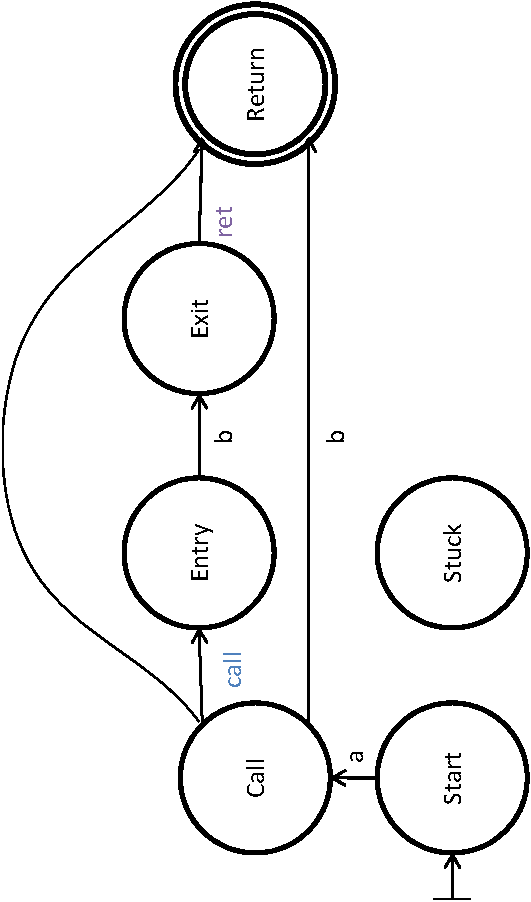
\includegraphics[angle=270,width=10cm]{Figures/Figure13.pdf}
%  \caption{Complex NWA on which to perform Kleene-Star.}
%  \label{Fi:Star3}
%\end{figure}

%\begin{figure}[htbp]
%  \centering
%    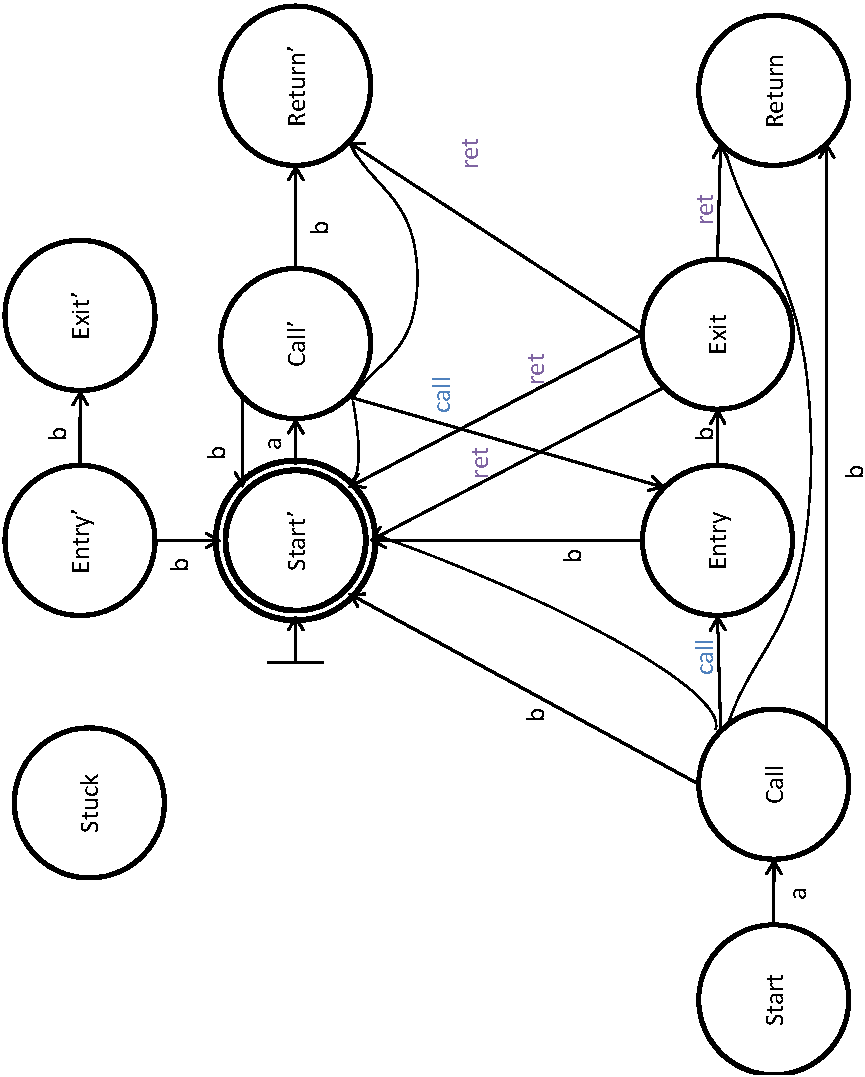
\includegraphics[angle=270,width=12cm]{Figures/Figure14.pdf}
%  \caption{The NWA resulting from performing Kleene-Star on the NWA in Figure \ref{Fi:Star3}.}
%  \label{Fi:Star4}
%\end{figure}

\subsection{Reverse}
\label{Se:Reverse}

The algorithm for reversing an NWA has a similar flavor to that of the Kleene
star procedure. The automaton $A^{rev}$ has two ``copies'' of $A$ (one
primed). The reversed automaton will start in the $A'$ copy, stay in $A'$
until it reads a call, transition to the $A$ copy, stay in $A$ until it reads
the matched return for the call that caused it to switch copies, then
transition back to $A'$.

Our construction of reverse is more complicated than the one presented in
\cite{JACM:AM2009}; this is necessary because the version in
\cite{JACM:AM2009} will not work as-stated with a weakly-hierarchical
NWA.

If the original NWA is $(Q, \Sigma, Q_0, \delta, Q_f)$, then the result of
reversing that NWA is $(Q \cup Q', \Sigma, Q_f', \delta^{rev}, Q_0)$ obtained using
the following rules:

\begin{mathpar}
{\inferrule*[left=\textsc{Internal}]
     { (p,\sigma,q) \in \delta_i  }
  { (q,\sigma,p)  \in \delta^{rev}_i \\ (q',\sigma,p')  \in \delta^{rev}_i }
} 
\and
{\inferrule*[left=\textsc{Call-Return}]
       { (q_c,\sigma_c,q_e) \in  \delta_c \\ (q_x,\_\!\_\,,\sigma_r,q_r) \in \delta_r }
  { (q_r, \sigma_r, q_x), (q_r', \sigma_r, q_x) \in \delta^{rev}_c \\
    (q_e, q_r, \sigma_c, q_c), (q_e, q_r', \sigma_c, q_c') \in \delta^{rev}_c }
}
\and
{\inferrule*[left=\textsc{Pending-Return}]
       { (q_c,\sigma,q_e) \in  \delta_c \\ q_f \in Q_f }
  { (q_e', q_f, \sigma, q_c') \in \delta^{rev}_R }
}
\end{mathpar}
%The \textsc{Pending-Return} rule is the most perplexing one. The name
%\textsc{Pending-Return} is written from the perspective of the reversed
%automaton -- in other words, the reversed automaton will take a transition
%added by this rule when it reads a pending return, and that pending return
%would have been a pending call in the original automaton. However, $q_f \in
%Q_f$ is written from the perspective of the original automaton: because
%$q_f$ is a final state in the original it is an initial state in the
%reversed automaton, and this is why the transition can be taken on a pending
%return.


The NWA resulting from performing reverse on the NWA shown in
Figure \ref{Fi:Example1} is shown in Figure \ref{Fi:Reverse1}.
 

Client
information is copied directly from the original NWA using
\texttt{ClientInfo::clone()}.

\subsection{Determinize}
\label{Se:Determinize}

\begin{definition}
An NWA, $(Q,\Sigma,Q_0,\delta,Q_f)$, is \textbf{deterministic} iff 

\begin{enumerate} 

\item $|Q_0| \leq 1$, 

\item For all $q \in Q$, there is never a choice between reading $\sigma$ and
  following a $\sigma$ transition or following a wild (\wild) transition:
  \begin{itemize}
    \item if $(q,\wild,q') \in \delta_i$ then $|\{q'|(q,\sigma,q') \in
      \delta_i, {\sigma\neq@}\}| = 0$; \\ otherwise, for all $\sigma \in \Sigma - \{\wild\}$,
      $|\{q'|(q,\sigma,q') \in \delta_i\}| \leq 1$,

    \item if $(q,\wild,q') \in \delta_c$ then $ |\{q'|(q,\sigma,q') \in
      \delta_c, {\sigma\neq@}\}| = 0$;\\
      otherwise, for all $\sigma \in \Sigma - \{\wild\}$,
      $|\{q'|(q,\sigma,q') \in \delta_c\}| \leq 1$, and

    \item for $q' \in Q$, if $(q,q',\wild,q'') \in \delta_r$ then
      $|\{q''|(q,q',\sigma,q'') \in \delta_r, {\sigma\neq@}\}| = 0$; \\
      otherwise, for all
      $\sigma \in \Sigma - \{\wild\}$, $|\{q''|(q,q',\sigma,q'') \in \delta_r\}|
      \leq 1$,
  \end{itemize}
\item There are no $\epsilon$ transitions:
 \begin{itemize}
   \item for all $(q,\sigma,q') \in \delta_i, \sigma \neq \epsilon$,
   \item for all $(q,\sigma,q') \in \delta_c, \sigma \neq \epsilon$, and
   \item for all $(q,q',\sigma,q'') \in \delta_r, \sigma \neq \epsilon$.
 \end{itemize}
\end{enumerate}
If an NWA is not deterministic, then it is \textbf{non-deterministic}.
\end{definition}

Determinizing an NWA operates like a
generalization of the classical subset construction.  Instead of the states
in the determinized NWA being subsets of states in the original NWA, states of the
determinized NWA are sets of state pairs (i.e., binary relations on states)
\cite{JACM:AM2009}.  To support determinization, the library provides a
typedef of \texttt{std::set$<$pair$<$State, State$>>$} as 
\texttt{NWA::BinaryRelation}. See also \texttt{wali/nwa/RelationOps.hpp}.

We present the algorithm we use for determinization in
\appref{DeterminizeAlgorithm}.

%There is very experimental support for using the BuDDY


The result of determinizing the automaton in \figref{Det1} is shown in
\figref{Det2}.

\begin{figure}[p]
  \centering
    \nwaimage[0.45]{Figures/determinize}
  \caption{Simple nondeterministic NWA.}
  \label{Fi:Det1}
\end{figure}


\begin{figure}[p]
  \centering
    \nwaimage[.75]{Figures/determinize-result}
    \caption{The NWA resulting from determinizing the NWA in Figure
      \ref{Fi:Det1}. As mentioned in the text, states in the determinized NWA
      are relations on the states in the original NWA. The state
      $\varnothing$ has been removed from this diagram.} 
  \label{Fi:Det2}
\end{figure}


Client information is generated through the use of the helper method
\texttt{mergeClientInfo}, but can be altered through the use of the helper
methods \texttt{mergeClientInfoInternal}, \texttt{mergeClientInfoCall}, and
\texttt{mergeClientInfoReturn}, which are invoked by \texttt{determinize} as
transitions of the three kinds involving the associated state are added.  The
default behavior of \texttt{mergeClientInfo} is that the \texttt{ClientInfo}
associated with the resulting state is \texttt{null}.  The default behavior
of \texttt{mergeClientInfoInternal}, \texttt{mergeClientInfoCall}, and
\texttt{mergeClientInfoReturn} is to make no changes to the the
\texttt{ClientInfo}.  These methods can be overridden to specify alternative
behaviors.  As determinization is performed, \texttt{mergeClientInfo} is
called each time a new state is created.  Then, as each transition is added,
\texttt{mergeClientInfoInternal}, \texttt{mergeClientInfoCall}, or
\texttt{mergeClientInfoReturn} is called (depending on the type of transition
being added) to update the \texttt{ClientInfo} associated with the target
state of the transition being added.

The following functions can be overridden in a subclass of \texttt{NWA} to
customize the behavior of determinization:
\begin{functionlist}
  \functionDefNoCloseParen{void}{mergeClientInfo}{%
     \parbox[t]{4in}{
       NWA const \& nondet, BinaryRelation const\& binRel, \\
       St resSt, ref\_ptr<ClientInfo>\& resCI)}}
  Callback that gets called when a new state \texttt{resSt} (representing the
  binary relation \texttt{binRel}) is added to the determinized automaton.
  Intended to provide a hook for computing the client information that should
  be associated with the new state; the client information should be set in
  the output parameter \texttt{resCI} (i.e., \texttt{setClientInfo} should not
  be called directly). \texttt{nondet} is the NWA being determinized.

  \functionDefFirstEarlyNoCloseParen{void}{mergeClientInfoInternal}{%
     \parbox[t]{4in}{
       NWA const \& nondet,\\
       BinaryRelation const\& binRelSource,\\
       BinaryRelation const\& binRelTarget,\\
       Key sourceSt, Key resSym, Key resSt,\\
       ref\_ptr<ClientInfo>\& resCI )}}
  \functionDefEarlyNoCloseParen{void}{mergeClientInfoCall}{%
     \parbox[t]{4in}{
       NWA const \& nondet,\\
       BinaryRelation const\& binRelCall,\\
       BinaryRelation const\& binRelEntry,\\
       Key callSt, Key resSym, Key resSt,\\
       ref\_ptr<ClientInfo>\& resCI )}}
  \functionDefNoCloseParen{void}{mergeClientInfoReturn}{%
     \parbox[t]{4in}{
       NWA const \& nondet,\\
       BinaryRelation const\& binRelExit,\\
       BinaryRelation const\& binRelCall,\\
       BinaryRelation const\& binRelReturn,\\
       Key exitSt, Key callSt, Key resSym,\\
       Key resSt, ref\_ptr<ClientInfo>\& resCI )}}
    Callbacks that get called when a new transition is added to the given
    automaton. The endpoints and their associated binary relations are
    given.
    Alters the client information associated with \texttt{resSt} given
    information about the transition being added to the determinized
    automaton.
 \end{functionlist}

%Consider the slightly more complex determinization of the NWA shown in Figure \ref{Fi:Det3}.  The resulting NWA is shown in Figure \ref{Fi:Det4}.

%\begin{figure}[htbp]
%  \centering
%    \includegraphics[angle=270,width=12cm]{Figures/Figure18.pdf}
%  \caption{Complex nondeterministic NWA.}
%  \label{Fi:Det3}
%\end{figure}

%\begin{figure}[htbp]
%  \centering
%    \includegraphics[angle=270,width=12cm]{Figures/Figure19.pdf}
%  \caption{The NWA resulting from determinizing the NWA in Figure \ref{Fi:Det3}.}
%  \label{Fi:Det4}
%\end{figure}

\subsection{Complement}
\label{Se:Complement}

Complementing an NWA is performed by determinizing the automaton and then
complementing the set of final states. In our implementation, an extra flag
to \texttt{complement} controls whether the determinization step is to be
performed, so it can be bypassed if you have \textsl{a priori} knowledge that
the input NWA must already be deterministic. The result of
complementing the NWA shown in Figure \ref{Fi:Det1} is
shown in Figure \ref{Fi:Comp1}.

Client information is copied directly
from the determinization of the original NWA using \texttt{ClientInfo::clone()}.

\begin{figure}[h]
  \centering
    \nwaimage[1]{Figures/complement-of-determinize}
  \caption{The complement of the NWA in Figure \ref{Fi:Det1} (the
    determinization of which is shown in Figure \ref{Fi:Det2}).  We omit
    transitions to the state $\{\}$; any action that does not appear in the
    diagram goes to the state $\{\}$.
  }
  \label{Fi:Comp1}
\end{figure}




\clearpage
\section{Conversions beween WPDSs and NWAs (namespace
  \texttt{wali::nwa::nwa\_pds})}
\label{Se:Conversions}


It is possible to convert a WALi WPDS to an NWA and vice versa.
However, the construction of an NWA from a WPDS is not the inverse
of constructing a WPDS from an NWA, i.e., one cannot perform the two
conversions in sequence and obtain the identity conversion.

At a high level, the WPDS to NWA conversion works by making the NWA encode both the state
of the WPDS and its top-of-stack symbol. A WPDS rule of the form $\langle
p,q_1 \rangle \hookrightarrow \langle p,q_2 \rangle$ leaves the stack height
unchanged, and is thus associated with an internal NWA transition; in this
case, that transition goes from the state $(p,q_1)$ to $(p,q_2)$. The symbol
of a transition is associated with the top-of-stack symbol of the source
state, so in this example, the symbol labeling that transition would be
$q_1$. In other words, the WPDS rule $\langle p,q_1 \rangle \hookrightarrow
\langle p,q_2 \rangle$ is translated to the NWA internal transition
$((p,q_1), q_1, (p,q_2))$.
WPDS push rules correspond to NWA call transitions, and WPDS pop rules
correspond to NWA return transitions.\footnote{
This encoding is motivated by our uses of both WPDSs and NWAs in program
analysis. It is common for WPDSs to have just one state, $p$, and to use the
top-of-stack symbol to encode the ``current'' program point. Pushing
something onto the stack corresponds to a call, and popping corresponds to a
return. For NWAs, we use the states themselves to encode the current program
point. (The function that
converts a WPDS into an NWA supports multi-state WPDSs, however; a WPDS rule
of the form $\langle p_1,q_1 \rangle \hookrightarrow
\langle p_2,q_2 \rangle$ is translated to the NWA internal transition
$((p_1,q_1), q_1, (p_2,q_2))$.)}

The conversion in the other direction creates a WPDS with one primary state
and one ``helper'' state for each NWA state that appears in the exit position
of a return transition. The NWA's state is encoded by the symbol at the top of the WPDS's
stack -- essentially the inverse of the encoding described in the previous
paragraph. A slight complication arises in the case of return
transitions. The NWA is able to look at both the exit node and the call
predecessor. In the WPDS this would correspond to looking at the top two stack
symbols -- but the WPDS is only allowed to look at the top \emph{one}. Hence each NWA return transition becomes
two WPDS rules: the first pops the top symbol (which corresponds to the
current NWA state) and remembers what it was using the helper state; the
second rule looks at the call predecessor and the helper state to dispatch to
the corresponding return site.

The library also offers two kinds of variants of this conversion. First, there
is a backwards variant that can be used for backwards dataflow-analysis
problems. Second, the resulting WPDS can stack either calls or returns. The
``stacking-calls'' version turns a call transition $(c, \sigma, e)$ into a
WPDS rule $\langle p, c\rangle \hookrightarrow \langle p, e c\rangle$ --
leaving the call predecessor $c$ on the stack. (This is the translation
described in the previous paragraph.) The ``stacking-returns'' version
has, in general, several WPDS push rules for each NWA call transition. Each
push rule leaves a potential return site on the stack. (For example, if there
is a call transition $(c,\sigma,e)$ and a return transition $(x, c, \sigma',
r)$, then the WPDS will have a rule $\langle p,
c\rangle\hookrightarrow\langle p, e r\rangle$).


The following functions are in the namespace \texttt{wali::nwa::nwa\_pds}
and, except for \texttt{plusWpds()}, are declared in the header
\texttt{wali/nwa/nwa\_pds/conversions.hpp}:


\begin{functionlist}
  \functionDefEarly{void}{WpdsToNwa}{NWA \& out, const WPDS\& pds}{}
  \functionDef{NWARefPtr}{WpdsToNwa}{const WPDS\& pds}{}
    Converts \texttt{pds} to an NWA, either storing the result in
    \texttt{nwa} or returning it.

\clearpage
  \functionDefFirstEarly{WPDS}{NwaToWpdsCalls}{NWA const \& nwa, WeightGen const \& wg}{}
  \functionDefEarlyNoCloseParen{WPDS}{NwaToWpdsCalls}{\parbox[t]{4in}{NWA const \& nwa, WeightGen const \& wg,\\ref\_ptr<Wrapper> wr)}}
  \functionDefEarly{WPDS}{NwaToBackwardsWpdsCalls}{NWA const \& nwa, WeightGen const \& wg}{}
  \functionDefEarly{WPDS}{NwaToWpdsReturns}{NWA const \& nwa, WeightGen const \& wg}{}
  \functionDef{WPDS}{NwaToBackwardsWpdsReturn}{NWA const \& nwa, WeightGen const \& wg}{}
    These functions each construct a WPDS that is equivalent to \texttt{nwa} using the
    appropriate method (backwards or forwards flow, and stacking calls or
    stacking returns), returning the result. Uses \texttt{wg} to determine
    weights for the WPDS's transitions. The second variant of
    \texttt{NwaToWpdsCalls} takes a \texttt{wali::wpds::Wrapper} reference
    \texttt{wr}, and the WPDS is constructed by passing \texttt{wr} to the
    constructor. This feature can be used, for instance, if you would like the
    resulting WPDS to support witness tracing. (If \texttt{wr} is
    \texttt{NULL}, then the second version is equivalent to the first.)

  \functionDefFirst{State}{getProgramControlLocation}{}{}
    Returns the program state $p$ used as the primary WPDS state in the
    result of the \texttt{NwaToWpds*} variants.

  \functionDefFirst{State}{getControlLocation}{State exit, State call, State return}{}
    Returns the WPDS state $p_{q_x}$ or $p_{q_3}$ used as a ``helper'' state
    for return transitions from \texttt{exit} to \texttt{return} with
    \texttt{call} as a predecessor.

  \functionDefFirst{WPDS}{plusWpds}{NWA const \& nwa, const WPDS\& base}{}
    This function returns a WPDS that is the
    product of the NWA \texttt{nwa} and WPDS \texttt{base}, as described in the ``Explicit
    NWA plus PDS'' construction from \cite[\S6]{advancedquerying}. This
    function is declared in the header
    \texttt{wali/nwa/nwa\_pds/plusWpds.hpp}.
\end{functionlist}


\subsection{WPDS to NWA}
\label{Se:WpdsToNwa}

The \texttt{WpdsToNwa} functions convert a WPDS into an NWA in a manner
faithful to the encoding sketched out in the introduction to this section.

Assume that we have a WPDS $(P, \Gamma, \Delta )$ 
where $\Delta = (\Delta_0, \Delta_1, \Delta_2)$. This 
WPDS is converted into an NWA $(Q,\Sigma,\{\},\delta,\{\})$ using the following rules:

\begin{mathpar}
{\inferrule*[left=\textsc{States}]
  { p \in P \\ q \in \Gamma }
  { (p,q) \in Q }
}
\and
{\inferrule*[left=\textsc{Alphabet}]
  { q \in \Gamma }
  { q \in \Sigma } 
}
\and 
\\
{\inferrule*[left=\textsc{Internal}]
  { \langle p,q \rangle \hookrightarrow \langle p',q' \rangle \in  \Delta_1 }
  { ( (p,q), q, (p',q') ) \in \delta_i  }
}
\and
{\inferrule*[left=\textsc{Call}]
  { \langle p,q_c \rangle \hookrightarrow \langle  p',q_e \hspace{.1cm} q_r \rangle \in \Delta_2 }
  { ( (p,q_c), q_c, (p',q_e) ) \in \delta_c }
} 
\and
{\inferrule*[left=\textsc{Return}]
  { \langle p'',q_x \rangle \hookrightarrow \langle p''',\epsilon  \rangle \in \Delta_0 \\
     \langle p,q_c \rangle \hookrightarrow \langle p',q_e \hspace{.1cm} q_r  \rangle \in \Delta_2 }
  { ( (p'',q_x), (p,q_c), q_x, (p''',q_r) ) \in \delta_r }
}
\end{mathpar}

Note that these rules generate an NWA return transition for each pair of WPDS pop
and push rules; there is no constraint between the two rules.  This is
because, with the exception of the ``revealed'' stack symbol $q_r$,
everything that the push rule talks about concerns the call predecessor
$(p,q_c)$ and entry node $(q', q_e)$; nothing that the pop rule talks about ---
$p''$, $q_x$, or $p'''$ --- has any relation to those. (A consequence is that the
number of NWA transitions may be quadratic in the number of
WPDS rules.)


In the resulting NWA, $Q_0$ and $Q_f$ are empty; client code must set the initial and
final states as appropriate (with \texttt{addInitialState(State)} and
\texttt{addFinalState(State)}. The keys that are generated for the names of the
NWA states are part of the interface of this function; they are generated by
\texttt{getKey(p, q)} where \texttt{p} and \texttt{q} are the keys of the
WPDS state and stack symbol being converted.

All weights on WPDS rules are ignored, and do not survive in any way in the
resulting NWA. The client information for all states in the resulting NWA are
set to \texttt{null}.


\begin{figure}[t]
  \centering
    \begin{itemize}
      \centering
      \item{ $\langle p,main \rangle \hookrightarrow \langle p,q_1 \rangle$}
      \item{ $\langle p,q_1 \rangle \hookrightarrow \langle p,c_1 \rangle$}
      \item{ $\langle p,c_1 \rangle \hookrightarrow \langle p,e \hspace{.1cm} r_1 \rangle$}
      \item{ $\langle p,e \rangle \hookrightarrow \langle p,q_2 \rangle$}
      \item{ $\langle p,q_2 \rangle \hookrightarrow \langle p,q_3 \rangle$}
      \item{ $\langle p,q_3 \rangle \hookrightarrow \langle p,x \rangle$}
      \item{ $\langle p,x \rangle \hookrightarrow \langle p,\epsilon \rangle$}
      \item{ $\langle p,r_1 \rangle \hookrightarrow \langle p,q_4 \rangle$}
      \item{ $\langle p,q_4 \rangle \hookrightarrow \langle p,q_5 \rangle$}
      \item{ $\langle p,q_5 \rangle \hookrightarrow \langle p,c_2 \rangle$}
      \item{ $\langle p,c_2 \rangle \hookrightarrow \langle p,e \hspace{.1cm} r_2 \rangle$}
      \item{ $\langle p,r_2 \rangle \hookrightarrow \langle p,q_6 \rangle$}
      \item{ $\langle p,q_6 \rangle \hookrightarrow \langle p,exit \rangle$}
    \end{itemize}
  \caption{An example WPDS.}
  \label{Fi:WpdsToNwa1}
\end{figure}

For example, the NWA created from the WPDS shown in
\figref{WpdsToNwa1} is shown in \figref{WpdsToNwa2}.

\begin{figure}[t]
  \centering
    \nwaimage[1]{Figures/pds-equivalent}
  \caption{The NWA resulting from converting the WPDS in \figref{WpdsToNwa1} into an NWA.}
  \label{Fi:WpdsToNwa2}
\end{figure}



\subsection{NWA to WPDS}
\label{Se:NWAtoPDS}


An NWA can also be converted into a WPDS. Weights for the rules of the
resulting WPDS are provided using a mechanism described below.  In this way
it is possible to use
the WPDS reachability queries that are a part of the main WALi library on
NWAs.  As mentioned in the introduction to \sectref{Conversions}, there are
four variations on the NWA-to-WPDS conversion: forward flow with call states
on the stack, backward flow with call states on the stack, forward flow with
return states on the stack, and backward flow with return states on the
stack. All four variations use \texttt{WeightGen} to determine weights for
WPDS rules.

\texttt{WeightGen} is an abstract class that client code must subclass to
calculate the weights of the rules in the generated WPDS.  It allows the
underlying NWA to be decoupled from the weight domain used in the WPDS.  See
\cite[\S4-\S5]{wali} for details about weight domains.

There is a trivial weight domain (containing $\overline{1}$ and
$\overline{0}$ only) implemented in the class \texttt{Reach}, defined in
\texttt{wali/Reach.hpp}. A \texttt{WeightGen} subclass that returns elements
from this reachability domain is provided as the \texttt{ReachGen} class,
defined in \texttt{wali/nwa/WeightGen.hpp}. \texttt{ReachGen} returns
$\overline{1}$ for all transitions.


\begin{figure}[p]
  \centering
  \begin{minipage}{\textwidth}
    \nwaimage[1]{Figures/pre-pds-nwa}
    \caption{An example NWA.}
    \label{Fi:NwaToWpds1}
  \end{minipage}
  \begin{minipage}{0.42\textwidth}
    \begin{itemize}
      \centering
      \item{ $\langle p,main \rangle \hookrightarrow \langle p,q_1 \rangle$}
      \item{ $\langle p,q_1 \rangle \hookrightarrow \langle p,c_1 \rangle$}
      \item{ $\langle p,e \rangle \hookrightarrow \langle p,q_2 \rangle$}
      \item{ $\langle p,q_2 \rangle \hookrightarrow \langle p,q_3 \rangle$}
      \item{ $\langle p,q_3 \rangle \hookrightarrow \langle p,x \rangle$}
      \item{ $\langle p,r_1 \rangle \hookrightarrow \langle p,q_4 \rangle$}
      \item{ $\langle p,q_4 \rangle \hookrightarrow \langle p,q_5 \rangle$}
      \item{ $\langle p,q_5 \rangle \hookrightarrow \langle p,c_2 \rangle$}
      \item{ $\langle p,r_2 \rangle \hookrightarrow \langle p,q_6 \rangle$}
      \item{ $\langle p,q_6 \rangle \hookrightarrow \langle p,exit \rangle$}
      \item{ $\langle p,c_1 \rangle \hookrightarrow \langle p,e \hspace{.1cm} c_1 \rangle$}
      \item{ $\langle p,c_2 \rangle \hookrightarrow \langle p,e \hspace{.1cm} c_2 \rangle$}
      \item{ $\langle p,x \rangle \hookrightarrow \langle p_x, \epsilon \rangle$}
      \item{ $\langle p_x,c_1 \rangle \hookrightarrow \langle p,r_1 \rangle$}
      \item{ $\langle p,x \rangle \hookrightarrow \langle p_x, \epsilon \rangle$}
      \item{ $\langle p_x,c_2 \rangle \hookrightarrow \langle p,r_2 \rangle$}
    \end{itemize}
    \caption{The WPDS resulting from calling \texttt{NwaToWpdsCalls} on \figref{NwaToWpds1}}
    \label{Fi:NwaToWpds4}
  \end{minipage}
  \hspace{0.1\textwidth}
  \begin{minipage}{0.42\textwidth}
    \centering
    \begin{itemize}
      \centering
      \item{ $\langle p,q_1 \rangle \hookrightarrow \langle p,main \rangle$}
      \item{ $\langle p,c_1 \rangle \hookrightarrow \langle p,q_1 \rangle$}
      \item{ $\langle p,q_2 \rangle \hookrightarrow \langle p,e \rangle$}
      \item{ $\langle p,q_3 \rangle \hookrightarrow \langle p,q_2 \rangle$}
      \item{ $\langle p,x \rangle \hookrightarrow \langle p,q_3 \rangle$}
      \item{ $\langle p,q_4 \rangle \hookrightarrow \langle p,r_1 \rangle$}
      \item{ $\langle p,q_5 \rangle \hookrightarrow \langle p,q_4 \rangle$}
      \item{ $\langle p,c_2 \rangle \hookrightarrow \langle p,q_5 \rangle$}
      \item{ $\langle p,q_6 \rangle \hookrightarrow \langle p,r_2 \rangle$}
      \item{ $\langle p,exit \rangle \hookrightarrow \langle p,q_6 \rangle$}
      \item{ $\langle p,r_1 \rangle \hookrightarrow \langle p,x \hspace{.1cm} r_1 \rangle$}
      \item{ $\langle p,r_2 \rangle \hookrightarrow \langle p,x \hspace{.1cm} r_2 \rangle$}
      \item{ $\langle p,e \rangle \hookrightarrow \langle p_e, \epsilon \rangle$}
      \item{ $\langle p_e,r_1 \rangle \hookrightarrow \langle p,c_1 \rangle$}
      \item{ $\langle p,e \rangle \hookrightarrow \langle p_e, \epsilon \rangle$}
      \item{ $\langle p_e,r_2 \rangle \hookrightarrow \langle p,c_2 \rangle$}
    \end{itemize}
    \caption{The result of calling \texttt{NwaToBackwardsWpdsCalls} on \figref{NwaToWpds1}}
    \label{Fi:NwaToWpds5}
  \end{minipage}
  \begin{minipage}{0.42\textwidth}
    \centering
    \begin{itemize}
      \centering
      \item{ $\langle p,main \rangle \hookrightarrow \langle p,q_1 \rangle$}
      \item{ $\langle p,q_1 \rangle \hookrightarrow \langle p,c_1 \rangle$}
      \item{ $\langle p,e \rangle \hookrightarrow \langle p,q_2 \rangle$}
      \item{ $\langle p,q_2 \rangle \hookrightarrow \langle p,q_3 \rangle$}
      \item{ $\langle p,q_3 \rangle \hookrightarrow \langle p,x \rangle$}
      \item{ $\langle p,r_1 \rangle \hookrightarrow \langle p,q_4 \rangle$}
      \item{ $\langle p,q_4 \rangle \hookrightarrow \langle p,q_5 \rangle$}
      \item{ $\langle p,q_5 \rangle \hookrightarrow \langle p,c_2 \rangle$}
      \item{ $\langle p,r_2 \rangle \hookrightarrow \langle p,q_6 \rangle$}
      \item{ $\langle p,q_6 \rangle \hookrightarrow \langle p,exit \rangle$}
      \item{ $\langle p,c_1 \rangle \hookrightarrow \langle p,e \hspace{.1cm} r_1 \rangle$}
      \item{ $\langle p,c_2 \rangle \hookrightarrow \langle p,e \hspace{.1cm} r_2 \rangle$}
      \item{ $\langle p,x \rangle \hookrightarrow \langle p_x, \epsilon \rangle$}
      \item{ $\langle p_x,r_1 \rangle \hookrightarrow \langle p,r_1 \rangle$}
      \item{ $\langle p,x \rangle \hookrightarrow \langle p_x, \epsilon \rangle$}
      \item{ $\langle p_x,r_2 \rangle \hookrightarrow \langle p,r_2 \rangle$}
    \end{itemize}
    \caption{The WPDS resulting from calling \texttt{NwaToWpdsReturns} on \figref{NwaToWpds1}}
    \label{Fi:NwaToWpds2}
  \end{minipage}
  \hspace{0.1\textwidth}
  \begin{minipage}{0.42\textwidth}
    \centering
    \begin{itemize}
      \centering
      \item{ $\langle p,q_1 \rangle \hookrightarrow \langle p,main \rangle$}
      \item{ $\langle p,c_1 \rangle \hookrightarrow \langle p,q_1 \rangle$}
      \item{ $\langle p,q_2 \rangle \hookrightarrow \langle p,e \rangle$}
      \item{ $\langle p,q_3 \rangle \hookrightarrow \langle p,q_2 \rangle$}
      \item{ $\langle p,x \rangle \hookrightarrow \langle p,q_3 \rangle$}
      \item{ $\langle p,q_4 \rangle \hookrightarrow \langle p,r_1 \rangle$}
      \item{ $\langle p,q_5 \rangle \hookrightarrow \langle p,q_4 \rangle$}
      \item{ $\langle p,c_2 \rangle \hookrightarrow \langle p,q_5 \rangle$}
      \item{ $\langle p,q_6 \rangle \hookrightarrow \langle p,r_2 \rangle$}
      \item{ $\langle p,exit \rangle \hookrightarrow \langle p,q_6 \rangle$}
      \item{ $\langle p,r_1 \rangle \hookrightarrow \langle p,x \hspace{.1cm} c_1 \rangle$}
      \item{ $\langle p,r_2 \rangle \hookrightarrow \langle p,x \hspace{.1cm} c_2 \rangle$}
      \item{ $\langle p,e \rangle \hookrightarrow \langle p_e, \epsilon \rangle$}
      \item{ $\langle p_e,c_1 \rangle \hookrightarrow \langle p,c_1 \rangle$}
      \item{ $\langle p,e \rangle \hookrightarrow \langle p_e, \epsilon \rangle$}
      \item{ $\langle p_e,c_2 \rangle \hookrightarrow \langle p,c_2 \rangle$}
    \end{itemize}
    \caption{The result of calling \texttt{Nwa\-To\-Backwards\-Wpds\-Returns} on \figref{NwaToWpds1}}
    \label{Fi:NwaToWpds3}
  \end{minipage}
\end{figure}


The following operations are virtual methods of \texttt{WeightGen} intended to
be overridden:

\begin{functionlist} 
  \functionDef{sem\_elem\_t}{WeightGen::getOne}{}{const = 0}  \nopagebreak
    Returns an instance of the $\bar{1}$ element of the weight domain.

  \functionDefFirstNoCloseParen{sem\_elem\_t}{getWeight}{%
      \parbox[t]{4in}{
        State source, ClientInfoRefPtr sourceInfo, \\  
        Symbol symbol, Kind k, \\
        State target, ClientInfoRefPtr targetInfo ) const}}  \nopagebreak
    Computes and returns the weight for the rule corresponding to the
    transition from \texttt{source} to \texttt{target} (of
    kind \texttt{k})
    labeled with symbol \texttt{symbol}. By default, returns \texttt{getOne()}.

  \functionDefFirstNoCloseParen{sem\_elem\_t}{getWildWeight}{%
      \parbox[t]{4in}{
        State source, ClientInfoRefPtr sourceInfo, \\  
        State target, ClientInfoRefPtr targetInfo ) const}}
    Computes and returns the weight for the WPDS rule corresponding to the
    transition from \texttt{source} to \texttt{target} labeled with the
    meta-symbol \wild. By default, returns \texttt{getOne()}.

  \functionDefFirst{sem\_elem\_t}{getExitWeight}{State src, ClientInfoRefPtr srcInfo}{const}
  This method computes the weight (in the desired semiring) for the return rule of
  the WPDS corresponding to the exit \texttt{src}.
  Note: the value is generally the same as \texttt{getOne()}, which is what the
  default implementation returns.

\end{functionlist}


\subsubsection{Forwards flow stacking calls}
\label{Se:wpds-forwards-flow-stacking-calls}

\noindent The conversion is performed by:



\begin{mathpar}

{\inferrule*%%[left=\textsc{States}]
  { }
  {p \in P}
}
\and 
{\inferrule*
  { (q_x,q_c,\sigma,q_r) \in \delta_r }
  { p_{q_x} \in P }
}
\and
{\inferrule*
  { q \in Q }
  { q \in \Gamma }
}
\and 
{\inferrule*%%[left=\textsc{Internal}]
  { (q,\sigma,q') \in \delta_i }
  { \langle p,q \rangle \stackrel{w_1}{\hookrightarrow} \langle p,q' \rangle \in \Delta_1 }
}
\and
{\inferrule*%%[left=\textsc{Call}]
  { (q_c,\sigma, q_e) \in \delta_c }
  {  \langle p,q_c \rangle \stackrel{w_2}{\hookrightarrow} \langle p, q_e \hspace{.1cm} q_c \rangle\in \Delta_2 }
}
\and
{\inferrule*%%[left=\textsc{Return}]
  { (q_x,q_c,\sigma,q_r) \in \delta_r }
  { \langle p,q_x \rangle \stackrel{w_0}{\hookrightarrow} \langle p_{q_x},\epsilon \rangle \in \Delta_0 \\
   \langle p_{q_x},q_c \rangle \stackrel{w_3}{\hookrightarrow} \langle p,q_r \rangle\in \Delta_1  }
}
\end{mathpar}
\begin{align*}
\text{where }
w_0 & = \begin{cases}
        \mathtt{wg.getOne}(), & \text{if } \sigma = \epsilon \\
        \mathtt{wg.getWildWeight}(q,CI_q,q',CI_{q'}), & \text{if } \sigma = \text{\wild} \\
        \mathtt{wg.getWeight}(q_x,CI_{q_x},\sigma,\mathtt{EXIT\_TO\_RET},q_r,CI_{q_r}), & \text{otherwise}
      \end{cases}  \\
w_1 &= \begin{cases}
         \mathtt{wg.getOne}(), & \text{if } \sigma = \epsilon \\
         \mathtt{wg.getWildWeight}(q,CI_q,q',CI_{q'}), & \text{if } \sigma = \text{\wild} \\
         \mathtt{wg.getWeight}(q,CI_q,\sigma,\mathtt{INTRA},q',CI_{q'}), & \text{otherwise}
      \end{cases} \\
w_2 &= \begin{cases}
         \mathtt{wg.getOne}(), & \text{if } \sigma = \epsilon \\
         \mathtt{wg.getWildWeight}(q,CI_q,q',CI_{q'}), & \text{if } \sigma = \text{\wild} \\
         \mathtt{wg.getWeight}(q_c,CI_{q_c},\sigma,\mathtt{CALL\_TO\_ENTRY},q_e,CI_{q_e}), & \text{otherwise}
      \end{cases} \\
w_3 &= \mathtt{wg.getOne}() 
\end{align*}


For example, the WPDS resulting from converting the NWA
shown in \figref{NwaToWpds1} into a WPDS is shown in
\figref{NwaToWpds4}. \\


\subsubsection{Backwards flow stacking calls}

The backwards-flow conversions are equivalent to calling
\texttt{wali::\-nwa::\-construct::\-reverse} and then the corresponding forwards
flow version. When reversing, call transitions become return transitions (and
vice versa), and so call sites become return sites (and vice versa).
Return sites in the original automaton behave as call sites in the reversed
automaton, and thus this version of the NWA-to-WPDS conversion stacks return
states. (In
other words, the \texttt{Calls} and \texttt{Returns} part of
\texttt{NwaTo\-Backwards\-WpdsCalls} and
\texttt{NwaTo\-Backwards\-WpdsReturns} refer to the behavior of the states in
the reversed automaton, not the role they play in the original.)

For example, the result of converting the NWA in
\figref{NwaToWpds1} into a backwards flow WPDS is shown in \figref{NwaToWpds5}.


Formally, the conversion is performed by:


\begin{mathpar}
{\inferrule*%%[left=\textsc{States}]
  { }
  {p \in P}
}
\and 
{\inferrule*
  { (q_c,\sigma,q_e) \in \delta_c }
  { p_{q_e} \in P }
}
\and
{\inferrule*
  { q \in Q }
  { q \in \Gamma }
}
\and 
{\inferrule*%%[left=\textsc{Internal}]
  { (q,\sigma,q') \in \delta_i }
  { \langle p,q' \rangle \stackrel{w_1}{\hookrightarrow} \langle p,q \rangle \in \Delta_1 }
}
\and  
{\inferrule*%%[left=\textsc{Call}]
  { (q_c,\sigma, q_e) \in \delta_c \\ (q_x,q_c,\gamma,q_r) \in \delta_r }
  { \langle p,q_e \rangle \stackrel{w_0}{\hookrightarrow} \langle p_{q_e},\epsilon \rangle \in \Delta_0 \\
    \langle p_{q_e},q_r \rangle \stackrel{w_3}{\hookrightarrow} \langle p,q_c  \rangle \in \Delta_1 }
}
\and
{\inferrule*%%[left=\textsc{Return}]
  { (q_x,q_c,\sigma,q_r) \in \delta_r }
  {  \langle p,q_r \rangle \stackrel{w_2}{\hookrightarrow} \langle p,q_x \hspace{.1cm} q_r
  \rangle \in \Delta_2 }
}
\end{mathpar}
\begin{align*}
\text{where }
w_0 &= \begin{cases}
           \mathtt{wg.getOne}(), & \text{if } \sigma = \epsilon \\
           \mathtt{wg.getWildWeight}(q_c,CI_{q_c},q_e,CI_{q_e}), & \text{if } \sigma = \text{\wild} \\
           \mathtt{wg.getWeight}(q_c,CI_{q_c},\sigma, \mathtt{CALL\_TO\_ENTRY},q_e,CI_{q_e}), & \text{otherwise}
      \end{cases} \\
w_1 &= \begin{cases}
           \mathtt{wg.getOne}(), & \text{if } \sigma = \epsilon \\
           \mathtt{wg.getWildWeight}(q,CI_q,q',CI_{q'}), & \text{if } \sigma = \text{\wild} \\
           \mathtt{wg.getWeight}(q,CI_q,\sigma, \mathtt{INTRA},q',CI_{q'}), & \text{otherwise}
       \end{cases} \\
w_2 &= \begin{cases}
          \mathtt{wg.getOne}(), & \text{if } \sigma = \epsilon \\
          \mathtt{wg.getWildWeight}(q_x,CI_{q_x},q_r,CI_{q_r}), & \text{if } \sigma = \text{\wild} \\
          \mathtt{wg.getWeight}(q_x,CI_{q_x},\sigma, \mathtt{EXIT\_TO\_RET},q_r,CI_{q_r}), & \text{otherwise}
      \end{cases} \\
w_3 &= \mathtt{wg.getOne}()
\end{align*}


\subsubsection{Forwards flow stacking returns}

As an example, converting the NWA in \figref{NwaToWpds1} into a WPDS results
in the WPDS shown in \figref{NwaToWpds2}. \\


The conversion is performed by:


\begin{mathpar}
{\inferrule*%%[left=\textsc{States}]
  { }
  {p \in P}
}
\and 
{\inferrule*
  { (q_x,q_c,\sigma,q_r) \in \delta_r }
  { p_{q_x} \in P }
}
\and
{\inferrule*
  { q \in Q }
  { q \in \Gamma }
}
\and 
{\inferrule*%%[left=\textsc{Internal}]
  { (q,\sigma,q') \in \delta_i }
  { \langle p,q  \rangle \stackrel{w_1}{\hookrightarrow} \langle p,q' \rangle \in \Delta_1 }
}
\and
{\inferrule*%%[left=\textsc{Call}]
  { (q_c,\sigma, q_e) \in \delta_c \\ (q_x,q_c,\gamma,q_r) \in \delta_r }
  { \langle p,q_c \rangle \stackrel{w_2}{\hookrightarrow}  \langle p, q_e \hspace{.1cm} q_r \rangle \in \Delta_2 }
}
\and 
{\inferrule*%%[left=\textsc{Return}]
  { (q_x,q_c,\sigma,q_r) \in \delta_r }
  { \langle p,q_x \rangle \stackrel{w_0}{\hookrightarrow} \langle p_{q_x},\epsilon \rangle \in  \Delta_0 \\
    \langle  p_{q_x},q_r \rangle \stackrel{w_3}{\hookrightarrow} \langle p,q_r \rangle \in \Delta_1 }
}
\end{mathpar}
\begin{align*}
\text{where }
w_0 &= \mathtt{wg.getOne}() \\
w_1 &= \begin{cases}
           \mathtt{wg.getOne}(), & \text{if } \sigma = \epsilon \\
           \mathtt{wg.getWildWeight}(q,CI_q,q',CI_{q'}), & \text{if } \sigma = \text{\wild} \\
           \mathtt{wg.getWeight}(q,CI_q,\sigma, \mathtt{INTRA},q',CI_{q'}), & \text{otherwise}
       \end{cases} \\
w_2 &= \begin{cases}
           \mathtt{wg.getOne}(), & \text{if } \sigma = \epsilon \\
           \mathtt{wg.getWildWeight}(q_c,CI_{q_c},q_e,CI_{q_e}), & \text{if } \sigma = \text{\wild} \\
           \mathtt{wg.getWeight}(q_c,CI_{q_c},\sigma, \mathtt{CALL\_TO\_ENTRY},q_e,CI_{q_e}), & \text{otherwise}
      \end{cases} \\
w_3 &= \begin{cases}
          \mathtt{wg.getOne}(), & \text{if } \sigma = \epsilon \\
          \mathtt{wg.getWildWeight}(q_x,CI_{q_x},q_r,CI_{q_r}), & \text{if } \sigma = \text{\wild} \\
          \mathtt{wg.getWeight}(q_x,CI_{q_x},\sigma, \mathtt{EXIT\_TO\_RET},q_r,CI_{q_r}), & \text{otherwise}
      \end{cases} 
\end{align*}




\subsubsection{Backwards flow stacking returns}

As an example, converting the NWA in
\figref{NwaToWpds1} into a backwards flow WPDS results in
the WPDS shown in \figref{NwaToWpds3}. \\


\noindent The conversion is performed by:



\begin{mathpar}
{\inferrule*[left=\textsc{States}]
  { }
  {p \in P}
}
\and 
{\inferrule*
  { (q_c,\sigma,q_e) \in \delta_c }
  { p_{q_e} \in P }
}
\and
{\inferrule*
  { q \in Q }
  { q \in \Gamma }
}
\and 
{\inferrule*%%[left=\textsc{Internal}]
  { (q,\sigma,q') \in \delta_i }
  { \langle  p,q' \rangle \stackrel{w_1}{\hookrightarrow} \langle p,q \rangle \in \Delta_1 }
}
\and
{\inferrule*%%[left=\textsc{Call}]
  { (q_c,\sigma, q_e) \in \delta_c }
  { \langle  p,q_e \rangle \stackrel{w_0}{\hookrightarrow} \langle p_{q_e},\epsilon \rangle \in \Delta_0 \\
    \langle  p_{q_e},q_c \rangle \stackrel{w_3}{\hookrightarrow} \langle p,q_c \rangle \in \Delta_1  }
}
\and 
{\inferrule*%%[left=\textsc{Return}]
  { (q_x,q_c,\sigma,q_r) \in \delta_r }
  { \langle p,q_r \rangle \stackrel{w_2}{\hookrightarrow} \langle p,q_x \hspace{.1cm} q_c  \rangle \in \Delta_2 }
}
\end{mathpar}
\begin{align*}
\text{where }
w_0 &= \mathtt{wg.getOne}() \\
w_1 &= \begin{cases}
           \mathtt{wg.getOne}(), & \text{if } \sigma = \epsilon \\
           \mathtt{wg.getWildWeight}(q,CI_q,q',CI_{q'}), & \text{if } \sigma = \text{\wild} \\
           \mathtt{wg.getWeight}(q,CI_q,\sigma, \mathtt{INTRA},q',CI_{q'}), & \text{otherwise}
       \end{cases} \\
w_2 &= \begin{cases}
          \mathtt{wg.getOne}(), & \text{if } \sigma = \epsilon \\
          \mathtt{wg.getWildWeight}(q_x,CI_{q_x},q_r,CI_{q_r}), & \text{if } \sigma = \text{\wild} \\
          \mathtt{wg.getWeight}(q_x,CI_{q_x},\sigma, \mathtt{EXIT\_TO\_RET},q_r,CI_{q_r}), & \text{otherwise}
      \end{cases} \\
w_3 &= \begin{cases}
           \mathtt{wg.getOne}(), & \text{if } \sigma = \epsilon \\
           \mathtt{wg.getWildWeight}(q_c,CI_{q_c},q_e,CI_{q_e}), & \text{if } \sigma = \text{\wild} \\
           \mathtt{wg.getWeight}(q_c,CI_{q_c},\sigma, \mathtt{CALL\_TO\_ENTRY},q_e,CI_{q_e}), & \text{otherwise}
      \end{cases} 
\end{align*}


\clearpage
\bibliographystyle{plain}
\bibliography{df,mab}
\clearpage
\appendix
\section{Nested-Word Automata and Overview of the Library's Organization}
\label{App:nwa-definition}

Nested-word automata (NWAs)~\cite{DLT:AM2006,JACM:AM2009} are a generalization
of finite-state automata that can capture the matched-parenthesis structure
that is exhibited by, for example, opening and closing tags in XML, and the
call/return structure in execution traces in multi-procedure
programs. Their languages represent somewhat of a middle-ground between
standard regular languages and context-free languages. Nested-word languages
retain the call/return structure mentioned above, which makes them a
refinement of standard regular languages. (For instance, there is an NWA that
accepts exactly the language of properly-balanced parentheses, with the
associated matching structure.) However, nested-word languages also retain all the closure
properties that makes standard regular languages attractive; in particular,
they are closed under complementation and intersection. However, they are not
directly comparable to languages of linear words, because the call/return
structure is an explicit part of each nested word.

\begin{definition}
  A \textsl{nested word} $(w,\rightsquigarrow)$ over alphabet $\Sigma$ is an
  ordinary (linear) word $w \in \Sigma^*$ of length $|w|$ together with a
  \textsl{nesting relation} $\rightsquigarrow$.

  The relation $\rightsquigarrow$ is a collection of edges (over the
  positions in $w$) that do not cross. Formally, $\rightsquigarrow \subseteq$
  $\{-\infty, 1, 2, \ldots, |w| \} \times \{1, 2, \ldots, |w|, +\infty\}$
  such that:
  \begin{itemize}
    \item
      Nesting edges only go forward: if $i \rightsquigarrow j$ then $i < j$.
    \item
      No two edges share a position unless one is $\pm\infty$: for $1
      \leq i \leq |w|$, either $i=\pm\infty$, $j=\pm\infty$, or
      there is at
      most one $j$ such that $i \rightsquigarrow j$ or $j \rightsquigarrow
      i$.
    \item
      Edges do not cross: if $i \rightsquigarrow j$ and $i' \rightsquigarrow
      j'$, then one cannot have $i < i' \leq j < j'$.
  \end{itemize}

  A \textsl{nested-word language} is any set of nested words; such a language
  is a \textsl{regular nested-word language} if it is accepted by an NWA as
  defined below.
\end{definition}

When $i \rightsquigarrow j$ holds, for $1 \leq i \leq |w|$, $i$ is called a
\textsl{call} position. If $i \rightsquigarrow +\infty$, then $i$ is a
\textsl{pending call}; otherwise $i$ is a \textsl{matched call}, and the
(unique) position $j$ such that $i \rightsquigarrow j$ is called its
\textsl{return successor}. (Note that these terms refer to positions within
$w$ rather than the symbol.)

Similarly, when $i \rightsquigarrow j$ holds, for $1 \leq j \leq |w|$, $j$
is a \textsl{return} position. If $-\infty \rightsquigarrow j$, then $j$ is
a \textsl{pending return}, otherwise $j$ is a \textsl{matched return}, and
the (unique) position $i$ such that $i \rightsquigarrow j$ is called its
\textsl{call predecessor}.

A position $1 \leq i \leq |w|$ that is neither a call nor a return is an
\textsl{internal} position.

A nested word is \textsl{balanced} if it has no pending calls
or returns.  A nested word is \textsl{unbalanced-left} (or a
\textsl{nested-word prefix}) if it has only pending calls, and it is
\textsl{unbalanced-right} (or a \textsl{nested-word suffix})
if it has only pending returns. (It is a general nested word otherwise.)


The library supports balanced and unbalanced-left nested words, but not
unbalanced-right.


\begin{definition}
  \label{De:NWA}

  A \textsl{nested-word automaton} (NWA) $A$ is a 5-tuple $(Q, \Sigma, Q_0,
  \delta, F)$, where $Q$ is a finite set of states, $\Sigma$ is a finite
  alphabet, $Q_0 \subseteq Q$ is the initial state, $F \subseteq Q$ is a set of
  final states, and $\delta$ is a transition relation. The transition
  relation $\delta$ consists of three components, $(\delta_c, \delta_i,
  \delta_r)$, where:
  \begin{itemize}
    \item
      $\delta_i: (Q \times \Sigma) \times Q$ is the transition relation for
      internal positions of the input word.
    \item
      $\delta_c: (Q \times \Sigma) \times Q$ is the transition relation for
      call positions.
    \item
      $\delta_r: (Q \times Q \times \Sigma) \times Q$ is the transition
      relation for return positions.
  \end{itemize}

  Starting from a state in $Q_0$, an NWA $A$ reads a nested word $(w,\rightsquigarrow)$
  from left to right, and performs transitions according to the current input
  symbol and $\rightsquigarrow$.  If $A$ is in state $q$ when reading input
  symbol $\sigma$ at position $i$ in $w$, and $i$ is an internal (resp, call)
  position in $\rightsquigarrow$, $A$ makes a transition to a state $q'$ (if
  one is available) such that $(q,\sigma,q')\in\delta_i$ (resp,
  $(q,\sigma,q')\in\delta_c$).  If $i$ is a return position, let $k$ be the
  call predecessor of $i$ (so $k \rightsquigarrow i$) and $q_c$ be the state
  $A$ was in just before the transition it made on the $k^{\textrm{th}}$
  symbol; $A$ changes to a state $q'$ such that $(q,q_c,\sigma,q')
  \in\delta_r$. If there is a computation of $A$ on input
  $(w,\rightsquigarrow)$ that terminates in a state $q\in F$, then $A$
  accepts $(w,\rightsquigarrow)$.

  NWAs can be either deterministic or nondeterministic, and these types have
  equivalent power.
\end{definition}


To distinguish among the different roles for states in an internal
transition $(q,\sigma,q')$, we say that $q$ is the source and $q'$ is the
target.  Similarly, to distinguish among the roles for states in a call
transition $(q_c,\sigma,q_e)$, we say that $q_c$ is the call state and $q_e$
is the entry state. To distinguish among the roles for states in a return
transition $(q_x,q_c,\sigma,q_r)$, we say that $q_x$ is the exit state,
$q_c$ is the call state (or call predecessor), and $q_r$ is the return state.

\clearpage
\section{Determinize}
\label{App:DeterminizeAlgorithm}

We found the explanations of how to determinize NWAs that are given
in~\cite{DLT:AM2006,JACM:AM2009} to be confusing (and contradictory between
the two accounts), and so we reformulated it using relational
operations.

We use the following notation in the determinize algorithm: \\
\begin{quote}
\begin{tabular}{ll}
  $(Q, \Sigma, \delta, Q_0, Q_f)$\hspace{1em}
                                     & The components of the input automaton \texttt{nwa} \\
  $\delta_i|_\sigma$                 & The binary relation $\{(p,q) | (p, \sigma, q) \in\delta_i\}$ \\
  $\delta_c|_\sigma$                 & The binary relation $\{(p,q) | (p, \sigma, q) \in\delta_c\}$ \\
  $\delta_r|_\sigma$                 & The binary relation $\{(p,q) | \exists c. (p, c, \sigma, q) \in\delta_r\}$ \\
  $R \circ S$                        & Relational composition of the binary relations $R$ and $S$ \\
  $R^*$                              & Transitive closure of the binary relation $R$ \\
  $Q^{new}, \delta^{new}$            & Components of the determinized NWA \\
\end{tabular}
\end{quote}
We use the following auxiliary function to compute the target of
a return transition:
\begin{eqnarray*}
  \textrm{Merge}(R^{exit}, R^{call}, \delta) = \{(q, q') & |& \exists q_1, q_2.\,(q, q_1) \in R^{call} \\
                                                         &&  \phantom{\exists q_1, q_2.\,}\textrm{and}\ (q_1, q_2) \in R^{exit} \\
                                                         &&  \phantom{\exists q_1, q_2.\,}\textrm{and}\ (q_2, q_1, q') \in \delta\}
\end{eqnarray*}

Each state $R$ in the determinized automaton is a binary relation on states
in the original. In a standard determinized FA, a state $\{q_0, q_1,
\cdots, q_n\}$ means the automaton can be in state $q_0$ of the original FA, or in
state $q_1$ of the original, etc. For NWAs, a state $\{(p_0, q_0), (p_1,
q_1), \cdots, (p_n, q_n)\}$ means that the NWA is one of the states $\{q_0,
q_1, \cdots, q_n\}$, but the relation carries around extra meaning.

If a state in the determinized automaton contains a pair $(p,q)$, then this
means the input automaton can begin in the state $p$, immediately take a call
transition, follow a path with balanced calls and returns, and finally arrive
in state $q$. In such a configuration, if the input automaton then reads a
return symbol, $q$ is the exit site and $p$ is the call predecessor. These
two pieces of information are exactly what the automaton needs to decide what
return transitions it can take. The call predecessor $p$ needs to be stored
explicitly because it is possible to arrive at the same state $q$ with
different call predecessors.

At the start of the run, and any time the automaton has not read any pending
calls, the first component of each pair in the current state will be some $q
\in Q_0$; this is because the initial states act as call predecessors in that
situation.

\newcommand{\WL}{\textit{WL}}

\newpage
\begin{algorithm}[H]
  \hrule
  \DontPrintSemicolon
  \SetAlgorithmName{Listing}{listing}{listing}
  \SetKw{Int}{int}
  \SetKw{Boolean}{bool}
  \SetKwBlock{DetDef}{determinize(NWA nwa)}{end}
  \SetKwFunction{Merge}{Merge}

  \DetDef{
    $Close$ = $(\delta_i |_\epsilon)^*$\;
    $Id$ = $\{(q,q) | q \in Q\}$\;
    $R_0$ = $Q_0 \times Q_0 \circ Close$\;
    $Q^{new}$ = $\{R_0\}$\;
    Insert $R_0$ in \WL\;
    \While{$\WL \neq \varnothing$}{
      select and remove a relation $R$ from \WL\;
      \tcp{Note that $R$ is a state in $Q^{new}$}
      mark $R$\;
      \For{$\sigma\in\Sigma$}{
        \tcp{Compute internal transitions}
        $R^i$ = $R \circ \delta_i|_\sigma \circ Close$\;
        $Q^{new}$ = $Q^{new} \cup \{R^i\}$\;
        Insert $R \overset{\sigma}{\rightarrow} R^i$ into $\delta_i^{new}$\;
        \If{$R^i$ unmarked}{
          $WL$ = $WL \cup \{R^i\}$\;
        }
        \BlankLine
        \tcp{Compute call transitions}
        $R^c$ = $Id \circ Close \circ \delta_c|_\sigma \circ Close$\;
        $Q^{new}$ = $Q^{new} \cup \{R^c\}$\;
        Insert $R \overset{\sigma}{\rightarrow} R^c$ into $\delta_c^{new}$\;
        \If{$R^c$ unmarked}{
          $WL$ = $WL \cup \{R^c\}$\;
        }
        \BlankLine
        \tcp{Compute return transitions where $R$ appears as the exit node}
        \For{$R^{call} \in Q^{new}$}{
          $R^r$ = $\Merge(R, R^{call}, \delta_r|_\sigma) \circ Close$\;
          $Q^{new}$ = $Q^{new} \cup \{R^r\}$\;
          Insert $(R, R^{call}, \sigma, R^r)$ into $\delta_r^{new}$\;
          \If{$R^r$ unmarked}{
            $WL$ = $WL \cup \{R^r\}$\;
          }
        }
        \BlankLine
        \tcp{Compute return transitions with $R$ as the call predecessor}
        \For{$R^{exit} \in Q^{new}$}{
          $R^r$ = $\Merge(R^{exit}, R, \delta_r|_\sigma) \circ Close$\;
          $Q^{new}$ = $Q^{new} \cup \{R^r\}$\;
          Insert $(R^{exit}, R, \sigma, R^r)$ into $\delta_r^{new}$\;
          \If{$R^r$ unmarked}{
            $WL$ = $WL \cup \{R^r\}$\;
          }
        }
      }
    }
    \tcp{end worklist while loop}
    $Q_f^{new}$ = $\{R \in Q^{new} |\ \textrm{there is}\ (p,q) \in R
                                      \ \textrm{with}\ q \in Q_f\}$\;
    \Return{$(Q^{new}, \Sigma, \delta^{new}, \{R_0\}, Q_f^{new})$}\;
  }
  \hrule
\end{algorithm}

\clearpage
\section{Tables}
\label{App:Tables}
This section provides a number of quick-reference tables.

The tables do not have \textsl{all} the information one needs to know in
order to call the functions, and the entries use some shorthands; but they
provide enough information for specifics to be looked up in the corresponding
header or Doxygen documentation. The caption of each table gives the header
that contains the functions listed. In the interest of space, the types of
the function arguments are sometimes omitted, but they are likely to be what you
expect.

\listoftables

\clearpage

\newgeometry{bottom=1in,top=0.7in}
\setlength{\extrarowheight}{4pt}

\begin{sidewaystable}\sffamily\footnotesize
\begin{threeparttable}
  \captionex{Accessors and mutators of NWA components}{All functions are
    members of the \texttt{NWA} class, and thus declared in
    \texttt{opennwa/NWA.hpp}.
}
\label{Ta:simple-functions}
\begin{tabular}{p{0.55in}p{1.40in}p{1.45in}p{1.2in}p{1.12in}p{1.05in}p{1.35in}}
\toprule
                 &  add\tnote{1}                            &  remove\tnote{1}                          &  check membership\tnote{2} &  count                &  clear                     &  get\tnote{3}                 \\
\hline\hline %---------------------------------------------------------------------------------------------------------------------------------------------------------------------------------------
states           &  addState(State st)                      &  removeState(State st)\tnote{4}           &  isState(State st)         &  sizeStates()         &  clearStates()\tnote{4}    &  getStates() or \newline
                                                                                                                                                                                             \{begin,end\}States()        \\
initial \newline
states           &  addInitialState(State st)               &  removeInitialState(State st)             &  isInitialState(State st)  &  sizeInitialStates()  &  clearInitialStates()      &  getInitialStates() or \newline
                                                                                                                                                                                             \{begin,end\}InitialStates() \\
final
\newline  states &  addFinalState(State st)                 &  removeFinalState(State st)               &  isFinalState(State)       &  sizeFinalStates()    &  clearFinalStates()        &  getFinalStates() or \newline
                                                                                                                                                                                             \{begin,end\}FinalStates()    \\
\hline %---------------------------------------------------------------------------------------------------------------------------------------------------------------------------------------
symbols\tnote{5} &  addSymbol(Symbol sym)                   &  removeSymbol(Symbol sym)\tnote{4}        &  isSymbol(Symbol sym)      &  sizeSymbols()        &  clearSymbols()            &  getSymbols() or \newline
                                                                                                                                                                                             \{begin,end\}Symbols()         \\
\hline %---------------------------------------------------------------------------------------------------------------------------------------------------------------------------------------
all \newline
transitions      &  ---                                     &  findTrans(State s1, \newline
                                                               \phantom{find}Symbol sym, State s2)&  ---                       &  sizeTrans()          &  clearTrans()              &  ---                           \\
internal \newline
transitions      &  addInternalTrans(\phantom{.}...\tnote{6}\phantom{a})
                                                            &  removeInternalTrans(\phantom{.}...\tnote{6}\phantom{a})
                                                                                                        &  ---                       &  sizeInternalTrans()  &  ---                       &  \{begin,end\}internalTrans()  \\
call \newline
transitions      &  addCallTrans(\phantom{.}...\tnote{6}\phantom{a})
                                                            &  removeCallTrans(\phantom{.}...\tnote{6}\phantom{a})
                                                                                                        &  ---                       &  sizeCallTrans()      &  ---                       &  \{begin,end\}callTrans()      \\
return \newline
transitions      &  addReturnTrans(\phantom{.}...\tnote{6}\phantom{a})
                                                            &  removeReturnTrans(\phantom{.}...\tnote{6}\phantom{a})
                                                                                                        &  ---                       &  sizeReturnTrans()  &  ---                       &  \{begin,end\}returnTrans()\\
\hline
\end{tabular}
\begin{tablenotes}
  \item[1] These functions return a \texttt{bool} indicating whether the item
    was added/removed. Adding a transition implicitly adds all
    states and symbols in that transition if they are not already present.
    Removing a state or symbol removes all transitions the removed item was a
    part of.
  \item[2] These functions return a \texttt{bool} with the natural
    interpretation.
  \item[3] The entries of the form, e.g., ``\{begin,end\}States()'' denote a pair
    of functions, each of which returns an iterator. The type of that iterator
    is either a \texttt{Nwa::StateIterator},
    \texttt{Nwa::SymbolIterator}, \texttt{Nwa::CallIterator},
    \texttt{Nwa::InternalIterator}, or \texttt{Nwa::ReturnIterator}, as appropriate; all of these are
    actually const iterators. The other functions (``get\textit{Kind}()'')
    return a \texttt{StateSet} or \texttt{SymbolSet} as appropriate.
  \item[4] Removing a state or a symbol also removes all transitions
    involving it. (Hence clearing all states or clearing all symbols also
    clears all transitions.)
  \item[5] \texttt{WALI\_EPSILON} and \texttt{WALI\_WILD} are not explicit
    members of the symbol set. This has the following consequences (for
    \texttt{s} as epsilon or wild): \texttt{addSymbol(s)} and
    \texttt{removeSymbol(s)} are both no-ops and return \texttt{false},
    \texttt{isSymbol(s)} returns false, \texttt{sizeSymbols()} does not count
    epsilon or wild, and neither the set returned by \texttt{getSymbols()}
    nor the iterator range \texttt{\{begin,end\}Symbols()} will contain
    epsilon or wild.
  \item[6] There are two overloads of each of these functions. The first
    takes each element of the transition tuple individually,
    e.g., \texttt{addCallTrans(State src, State sym, State tgt)}. The
    second takes a (constant reference to an) \texttt{Nwa::Internal},
    \texttt{Nwa::Call}, or \texttt{Nwa::Return} object (as
    appropriate). (These are typedefs of a \texttt{Triple} or \texttt{Quad}
    of the appropriate type.)
\end{tablenotes}
\end{threeparttable}
\end{sidewaystable}



\newcommand{\RP}{\tnote{1}} %"returns pair"

\begin{sidewaystable}\sffamily
\begin{threeparttable}
\captionex{Query functions for all transition types}{These functions are
  in the namespace \texttt{opennwa::query}; include the
  file \texttt{opennwa/query/transitions.hpp}. For return transitions, the
  ``source'' is the first component of the transition; nothing involving call
  predecessors (the second component of return transitions) appears in this table. A table
  entry of ``---'' means that the combination of arguments does not make sense.
}
\label{Ta:query-all-transitions}
\begin{tabular}{p{1in}p{1in}|@{\hspace{0.1in}}p{2.2in}p{2.2in}p{2in}}
\toprule\toprule
\multicolumn{2}{c|@{\hspace{0.1in}}}{\textsl{What you know}} & \multicolumn{3}{c}{\textsl{What you want}}                                                                 \tabularnewline
 this...        & ... and this      &    sources                    &   symbols                          &    targets                     \tabularnewline
\midrule
\midrule %-------------------------------------------------------------------------------------------------------------------------------
  source        &  (nothing)        &      ---                      &  (none)                            &  getSuccessors(nwa, src)       \tabularnewline
                &  symbol           &      ---                      &        ---                         &  getSuccessors(nwa, src, sym)  \tabularnewline
                &  target           &      ---                      &  getSymbol(nwa, src, tgt, \&sym)   &   ---                          \tabularnewline
\midrule %-------------------------------------------------------------------------------------------------------------------------------
  symbol        &  (nothing)        &      ---                      &        ---                         &   (none)                       \tabularnewline
                &  target           & getPredecessors(nwa, sym, tgt)&       ---                         &   ---                          \tabularnewline
\midrule %-------------------------------------------------------------------------------------------------------------------------------
  target        &  (nothing)        & getPredecessors(nwa, tgt)     &  (none)                            &   ---                          \tabularnewline
\bottomrule\bottomrule
\end{tabular}
\end{threeparttable}
\end{sidewaystable}

\begin{sidewaystable}\sffamily
\captionex{Query functions for internal transitions.}{%
  These functions are in the namespace \texttt{opennwa::query};
  include the file \texttt{opennwa/query/internals.hpp}.
  A table entry of ``---'' means that combinations of arguments does not make
  sense.
}
\label{Ta:query-internal-transitions}
\begin{threeparttable}
\begin{tabular}{p{1in}p{1in}|@{\hspace{0.1in}}p{2.2in}p{2.2in}p{2in}}
\toprule\toprule
\multicolumn{2}{c|@{\hspace{0.1in}}}{\textsl{What you know}} & \multicolumn{3}{c}{\textsl{What you want}}                                                                 \tabularnewline
 this...        & ... and this      &    sources                    &   symbols                          &    targets                     \tabularnewline
\midrule
\midrule %-------------------------------------------------------------------------------------------------------------------------------
 (nothing)      &  (nothing)        & getSources(nwa)               &  getInternalSym(nwa)               &  getTargets(nwa)               \tabularnewline
\midrule %-------------------------------------------------------------------------------------------------------------------------------
  source        &  (nothing)        &      ---                      &  getInternalSym\_Source(nwa, src) \newline
                                                                       or getTargets(nwa, src)\RP        &  getTargets(nwa, src)\RP       \tabularnewline
                &  symbol           &      ---                      &        ---                         &  getTargets(nwa, src, sym)     \tabularnewline
                &  target           &      ---                      &  getInternalSym(nwa, src, tgt)     &   ---                          \tabularnewline
\midrule %-------------------------------------------------------------------------------------------------------------------------------
  symbol        &  (nothing)        & getSources\_Sym(nwa, sym)     &        ---                         &  getTargets\_Sym(nwa, sym)     \tabularnewline
                &  target           & getSources(nwa, sym, tgt)     &        ---                         &   ---                          \tabularnewline
\midrule %-------------------------------------------------------------------------------------------------------------------------------
  target        &  (nothing)        & getSources(nwa, tgt)\RP       &  getInternalSym\_Target(nwa, tgt) \newline
                                                                       or getSources(nwa, tgt)\RP        &   ---                          \tabularnewline
\bottomrule\bottomrule
\end{tabular}
\begin{tablenotes}
  \item[1] Returns a set of pairs (either source/symbol or symbol/target).
\end{tablenotes}
\end{threeparttable}
\end{sidewaystable}

\begin{sidewaystable}\sffamily
\begin{threeparttable}
\captionex{Query functions for call transitions}{These functions are in the
  namespace \texttt{opennwa::query}; include the
  file \texttt{opennwa/query/calls.hpp}. The ``call site'' is the source of the transition (and uses the argument 
  name \texttt{call}), and the ``entry'' of the transition is the target (and
  uses the argument name \texttt{ent}).
}
\label{Ta:query-call-transitions}
\begin{tabular}{p{1in}p{1in}|@{\hspace{0.1in}}p{2.2in}p{2.2in}p{2in}}
\toprule\toprule
\multicolumn{2}{c|@{\hspace{0.1in}}}{\textsl{What you know}} & \multicolumn{3}{c}{\textsl{What you want}}                                                                 \tabularnewline
 this...        & ... and this      &    call sites                   &   symbols                          &    entries                     \tabularnewline
\midrule
\midrule %-------------------------------------------------------------------------------------------------------------------------------
 (nothing)      &  (nothing)        & getCallSites(nwa)               &  getCallSym(nwa)                   &  getEntries(nwa)               \tabularnewline
\midrule %-------------------------------------------------------------------------------------------------------------------------------
 call site      &  (nothing)        &      ---                        &  getCallSym\_Call(nwa, call)\newline
                                                                         or getEntries(nwa, call)\RP       &  getEntries(nwa, call)\RP      \tabularnewline
                &  symbol           &      ---                        &        ---                         &  getEntries(nwa, call, sym)    \tabularnewline
                &  target           &      ---                        &  getCallSym(nwa, call, ent)        &   ---                          \tabularnewline
\midrule %-------------------------------------------------------------------------------------------------------------------------------
  symbol        &  (nothing)        & getCallSites\_Sym(nwa, sym)     &        ---                         &  getEntries\_Sym(nwa, sym)     \tabularnewline
                &  target           & getCallSites(nwa, sym, ent)     &        ---                         &   ---                          \tabularnewline
\midrule %-------------------------------------------------------------------------------------------------------------------------------
  entry         &  (nothing)        & getCallSites(nwa, ent)\RP       &  getCallSym\_Entry(nwa, ent) \newline
                                                                         or getCallSites(nwa, ent)\RP      &   ---                          \tabularnewline
\bottomrule\bottomrule
\end{tabular}
\begin{tablenotes}
  \item[1] Returns a set of pairs (either call site/symbol or symbol/entry).
\end{tablenotes}
\end{threeparttable}
\end{sidewaystable}

\begin{sidewaystable}\footnotesize\sffamily
\begin{threeparttable}
\captionex{Query functions for return transitions.}{These functions are in the
  namespace \texttt{opennwa::query}; include the
  file \texttt{opennwa/query/returns.hpp}.   The ``exit site'' is the source of the transition
  (the first component) and uses the argument name \texttt{exit} in this table;
  the ``call predecessor'' is the second component and uses the argument
  name \texttt{call}; the symbol is the third component and uses the argument
  name \texttt{sym}; the ``return site'' is the fourth component and uses the
  argument name \texttt{ret}.
}
\label{Ta:query-return-transitions}
\begin{tabular}{p{0.5in}p{0.55in}p{0.5in}|@{\hspace{0.1in}}p{1.55in}p{1.7in}p{1.7in}p{1.75in}}
\toprule\toprule
\multicolumn{3}{c|@{\hspace{0.1in}}}{\textsl{What you know}}  & \multicolumn{4}{c}{\textsl{What you want}}                                                                                                                                                \tabularnewline
 this...  & and this ...  & and this & exit sites & call predecessors &
 symbols & return sites \tabularnewline
\midrule
\midrule %--------------------------------------------------------------------------------------------------------------------------------------------------------------------------------------------------------------------
 (nothing)      &  (nothing)        &  (nothing)    & getExits(nwa)                 &  getCalls(nwa)                        &  getReturnSym(nwa)                           &  getReturns(nwa)                            \tabularnewline
\midrule %--------------------------------------------------------------------------------------------------------------------------------------------------------------------------------------------------------------------
 exit site      &  (nothing)        &  (nothing)    &      ---                      &  getCalls\_Exit(nwa, exit)\RP         &  getReturnSym\_Exit(nwa, exit) \newline
                                                                                                                               or getReturns\_Exit(nwa, exit)\RP\newline
                                                                                                                               or getCalls\_Exit(nwa, exit)\RP             &  getReturns\_Exit(nwa, exit)\RP             \tabularnewline
                \cline{2-7} %-------------------------------------------------------------------------------------------------------------------------------------------------------------------------------------------------
                &  call pred        &  (nothing)    &      ---                      &    ---                                &  getReturnSym\_ExitCall(nwa, exit, \newline
                                                                                                                               \phantom{getReturnSym\_ExitCall(}call) \newline
                                                                                                                               or getReturns(nwa, exit, call)\RP           &  getReturns(nwa, exit, call)\RP             \tabularnewline
                &                   &  symbol       &      ---                      &    ---                                &        ---                                   &  getReturns(nwa, exit, call, sym)           \tabularnewline
                &                   &  return       &      ---                      &    ---                                &  getReturnSym(nwa, exit, call, \newline
                                                                                                                               \phantom{getReturnSym(}ret)                 &    ---                                      \tabularnewline
                \cline{2-7} %-------------------------------------------------------------------------------------------------------------------------------------------------------------------------------------------------
                &  symbol           &  (nothing)    &      ---                      &  getCalls\_Exit(nwa, exit, sym)       &        ---                                   &  getReturns\_Exit(nwa, exit, sym)           \tabularnewline
                &                   &  return       &      ---                      &  getCalls(nwa, exit, sym, ret)        &        ---                                   &  getEntries(nwa, call, sym, ret)            \tabularnewline
                \cline{2-7} %-------------------------------------------------------------------------------------------------------------------------------------------------------------------------------------------------
                &  return site      &  (nothing)    &      ---                      &  getCalls(nwa, exit, ret)\RP          &  getReturnSym\_ExitRet(nwa, exit, \newline
                                                                                                                               \phantom{getReturnSym\_ExitRet(}ret) \newline
                                                                                                                               or getCalls(nwa, exit, ret)\RP              &   ---                                       \tabularnewline
\midrule %-------------------------------------------------------------------------------------------------------------------------------------------------------------------------------------------------------------------
 call pred      &  (nothing)        &  (nothing)    & getExits\_Call(nwa, call)\RP  &   ---                                 &  getReturnSym\_Call(nwa, call) \newline
                                                                                                                               or getReturns\_Call(nwa, call)\RP\newline
                                                                                                                               or getExits\_Call(nwa, call)\RP            &  getReturnSites(nwa, call) or \newline
                                                                                                                                                                             getCallSuccessors(nwa, call) or \newline
                                                                                                                                                                             getReturns\_Call(nwa, call)\RP              \tabularnewline
                \cline{2-7} %-------------------------------------------------------------------------------------------------------------------------------------------------------------------------------------------------
                &  symbol           &  (nothing)    & getExits\_Call(nwa, call, sym)&   ---                                 &        ---                                   &  getCallSuccessors(nwa, call, sym) \newline
                                                                                                                                                                              or getReturns\_Call(nwa, call, sym)        \tabularnewline
                &                   &  return       & getExits(nwa, call, sym, ret) &   ---                                 &        ---                                   &    ---                                      \tabularnewline
                \cline{2-7} %-------------------------------------------------------------------------------------------------------------------------------------------------------------------------------------------------
                &  return site      &  (nothing)    & getExits(nwa, call, ret)\RP   &   ---                                 &  getReturnSym\_CallRet(nwa, call, \newline
                                                                                                                               \phantom{getReturnSym\_CallRet(}ret) \newline
                                                                                                                               or getExits(nwa, call, ret)\RP              &   ---                                       \tabularnewline
\midrule %--------------------------------------------------------------------------------------------------------------------------------------------------------------------------------------------------------------------
 symbol         &  (nothing)        &  (nothing)    & getExits\_Sym(nwa, c)         &  getCalls\_Sym(nwa, c)                &   ---                                        &  getReturns\_Sym(nwa, sym)                  \tabularnewline
                \cline{2-7} %-------------------------------------------------------------------------------------------------------------------------------------------------------------------------------------------------
                &  return site      &  (nothing)    & getExits\_Ret(nwa, call, ret) &  getCallPredecessors(nwa, sym, ret) \newline
                                                                                       or getCalls\_Ret(nwa, sym, c)        &   ---                                        &   ---                                       \tabularnewline
\midrule %--------------------------------------------------------------------------------------------------------------------------------------------------------------------------------------------------------------------
 return site    &  (nothing)         & (nothing)    & getExits\_Ret(nwa, ret)       &  getCallPredecessors(nwa, ret) \newline
                                                                                       or getCalls\_Ret(nwa, ret)\RP        &  getReturnSym\_Ret(nwa, ret) or \newline
                                                                                                                               getCalls\_Ret(nwa, ret)\RP                  &   ---                                       \tabularnewline
\bottomrule\bottomrule
\end{tabular}
\begin{tablenotes}
  \item[1] Returns a set of pairs (a symbol with one of the states, in the order of the raw transition).
\end{tablenotes}
\end{threeparttable}
\end{sidewaystable}
\restoregeometry


\end{document}
